\section*{Learning Objectives}
\begin{itemize}
\item A second encounter with some of the essential concepts in Linear Algebra.
\item A more abstract view of $\real^n$ as a vector space.
\end{itemize}

\section*{Outcomes}
\begin{itemize}
\item What is a vector space, a subspace, and the span of a set of vectors.
\item Range, column span, and null space of a matrix.
\item The dot product and orthogonality.
\item Gram Schmidt process for generating a basis consisting of orthogonal vectors
\item Orthogonal matrices: they have the magical property that their inverse is the matrix transpose.
\item The QR Factorization is the most numerically robust method for solving systems of linear equations. 
\item Our second recommended ``pipeline'' (CS-speak for method) for solving $Ax=b$.
\end{itemize}

\vspace*{2cm}

\begin{tcolorbox}[sharp corners, colback=yellow!30, colframe=yellow!80!red, title=\textcolor{red}{\Large \bf Reminder: Additional Study Time May Be Required}] 
\bf For many students, the concepts in Chapters \ref{chap:Chap07VectorSpaceRnPart1}, \ref{chap:Rnpart2} and \ref{chap:matrixFacts} are significantly more challenging than the material in any of the other chapters of the book. Why? Well, the reasons vary from person to person, but the biggest reason seems to be the level of abstraction. All of our previous work has pretty much dealt with solving equations and that is something most students of ROB 101 can wrap their heads around.
\end{tcolorbox}


\newpage
\section{Motivation}

Up to this point, everything we have studied has been built around the notion of solving systems of linear equations. We found that it is very powerful to express linear equations in terms of matrices and vectors, namely in the form $Ax=b$. While $x$ is really a vector of ``unknowns'', we've become so comfortable with the vector $x$ being an object in and of itself that we're perfectly content to call $x$ ``the unknown''. Likewise, we're content to think of the matrix $A$ as an object, and even though it may be $50 \times 50$ and hence have $2,500$ individual entries, we've learned that moving our attention away from the individual entries to the bigger object, namely the matrix formed by the entries, is a very useful and powerful idea for solving equations.\\

Being able to think in terms of vectors and matrices was a big step in the level of abstraction from how we initially expressed equations in Chapter~\ref{chap:Intro}. For those of you who had seen matrices in High School, you took it in stride and thought for sure we'd be doing eigenvalues and eigenvectors pretty soon, though you would not have been able to say why studying them would be important for engineers, and for sure, you did not see triangular matrices, LU Factorization, and least-squared-error solutions coming nor how these tools would allow us to solve (exactly or approximately) equations with hundreds, or even thousands of variables. For those of you who had not seen matrices and vectors in High School, it was initially very hard to grasp the idea of vectors and matrices, but once you had accepted them as valid mathematical objects, you got to immediately manipulate them in Julia instead of only doing hand calculations. By working with vectors and matrices in a programming language, you could associate them with doing ``math at the scale of life'' instead of the tedium, not to mention the high chance of error, of doing hand calculations with vectors and matrices. And when we said ``NOPE'' to formulas for computing determinants or matrix inverses for general square matrices, but instead took a structured approach through triangular matrices and factorizations, you probably thought, yeah, this is how it is supposed to be done, and you were right! \\

In this Chapter, we take another big step in the level of abstraction. In fact, it's a really big step. Instead of looking at a given set of vectors or a particular linear combination formed from a set of vectors, we will look at the ``set of all possible linear combinations'' that one can generate from the set of vectors! Or, instead of looking at one solution to a set of linear equations, we will look at the ``set of all possible solutions'' to the set of equations! Why in the world would we ever want to do that? You're probably saying to yourself, `` the payoffs better be worth it, because, just thinking about the term \textit{all possible} is hurting my brain!'' \\

For sure. Now, back in Chapter~\ref{chap:Chap02VectorsMatricesDeterminants}, if we had tried to foreshadow everything we would be able to do with vector and matrices, you would have been overwhelmed. In fact, some of you may have sought a different course altogether. We'll take a chance that you are now more mathematically sophisticated and can handle the truth. If you are not so sure, you can stop here and begin Chapter~\ref{sec:VectorSpace}.

\begin{enumerate}
\renewcommand{\labelenumi}{(\alph{enumi})}
\setlength{\itemsep}{.2cm}
    \item When we form all possible linear combinations from a set of vectors that live in $\real^n$, we'll generate a subset of $\real^n$ called a \textit{subspace}. We'll come to realize that we can sort of go back and forth between this larger set, namely the subspace, and the original set of vectors. Now, once we have accepted the existence of this larger set called a subspace, we will ask the questions, ``Can a different set of vectors generate the same subspace that we generated from our original vectors? And if so, could these vectors be simpler to work with, or ``better'' in some sense?'' The answers will be ``yes'' and ``yes''! This will lead us to the \textit{QR Factorization} of a matrix, one of the most recommended\footnote{The world's leading experts argue back and forth over which is better: QR or LU? The QR Factorization is often better in the face of the numerical errors that arise from representing numbers in digital computers via a finite set of zeros and ones, while in many situations, the LU Factorization can be faster to compute, and hence allow one to solve larger problems. } methods for computing solutions to large systems of linear equations, the other being the \textit{LU Factorization}.
    
    \item So far in ROB 101, we have not come to grips with how to treat systems of linear equations $Ax=b$ that have an infinite number of solutions! We'll look at the set of all possible solutions and realize that it can be formed by knowing any particular solution to the equation, say $A \overline{x} = b$, and a subspace called the \textit{null space} of $A$. We'll then search within the set of all possible solutions for a solution having minimum norm. In Project 3, you'll use this idea to balance a Segway! Here, we'll not do anything so cool. 
\end{enumerate} 


\section{$\real^n$ as a Vector Space}
\label{sec:VectorSpace}

Let's recall that an $n$-tuple is a fancy name for an ordered list of $n$ numbers, $(x_1, x_2, \ldots, x_n)$ and that we typically identify them with column vectors, as in 
$$(x_1, x_2, \ldots, x_n) \longleftrightarrow \begin{bmatrix} x_1 \\ x_2 \\ \vdots \\ x_n\end{bmatrix}. $$
Moreover, we identify $\real^n$ with the set of all $n$-column vectors with real entries
$$
\{(x_1, x_2, \ldots, x_n)~|~x_i \in \real, 1\le i \le n \} \iff \real^n \iff  \left\{\begin{bmatrix} x_1 \\ x_2 \\ \vdots \\ x_n\end{bmatrix} ~\Bigg|~  x_i \in \real, 1\le i \le n \right\}
$$
Finally, the choice of identifying $n$-tuples of numbers with column vectors instead of row vectors is completely arbitrary, and yet, we have to choose one or the other when doing computations, and the most common choice is to use column vectors.

\begin{tcolorbox}
Two absolutely key properties of vectors in $\real^n$ is that we know how to add them and obtain another vector in $\real^n$, namely
\begin{equation}
    \label{eq:RnClosedUnderVectorAddition}
  \begin{bmatrix} x_1 \\ x_2 \\ \vdots \\ x_n\end{bmatrix} + 
 \begin{bmatrix} y_1 \\ y_2 \\ \vdots \\ y_n\end{bmatrix} :=
   \begin{bmatrix} x_1 + y_1\\ x_2 + y_2 \\ \vdots \\ x_n + y_n\end{bmatrix},
\end{equation}
and we know how to multiply a scalar times a vector and obtain another vector in $\real^n$, namely
\begin{equation}
    \label{eq:RnClosedUnderScalarTimesVectorMultiplication}
  \alpha \cdot \begin{bmatrix} x_1 \\ x_2 \\ \vdots \\ x_n\end{bmatrix} 
  :=
   \begin{bmatrix} \alpha x_1 \\ \alpha x_2 \\ \vdots \\ \alpha x_n\end{bmatrix}.
\end{equation}
Equation \eqref{eq:RnClosedUnderVectorAddition} says that the sum of two vectors is DEFINED by the sum of their respective components using the definition of addition of real numbers. Equation \eqref{eq:RnClosedUnderScalarTimesVectorMultiplication} says that the product of a scalar and a vector is DEFINED by the multiplication of the real numbers constituting the components of the vector by the scalar, which is another real number. It is emphasized that the vector operations are defined in terms the elementary operations of addition and multiplication of real numbers.\\

\textbf{Now, \eqref{eq:RnClosedUnderVectorAddition} and \eqref{eq:RnClosedUnderScalarTimesVectorMultiplication} are special cases of linear combinations. In fact, the following statements are equivalent (means, one holds if, and only if, the other holds)}
\begin{enumerate}
\renewcommand{\labelenumi}{(\alph{enumi})}
\setlength{\itemsep}{.2cm}

\item For all real numbers $\alpha$ and $\beta$, and all vectors $x$ and $y$ in $\real^n$
\begin{equation}
    \label{eq:RnClosedUnderLinearCombinations}
    \alpha  \begin{bmatrix} x_1 \\ x_2 \\ \vdots \\ x_n\end{bmatrix} + \beta
 \begin{bmatrix} y_1 \\ y_2 \\ \vdots \\ y_n\end{bmatrix} =
   \begin{bmatrix} \alpha x_1 + \beta y_1\\ \alpha x_2 + \beta y_2 \\ \vdots \\ \alpha x_n + \beta y_n\end{bmatrix}
   \end{equation}
   
   \item Both \eqref{eq:RnClosedUnderVectorAddition} and \eqref{eq:RnClosedUnderScalarTimesVectorMultiplication} hold individually.
\end{enumerate}
\end{tcolorbox}

\textbf{Remark:} To see the equivalency, note that  if in \eqref{eq:RnClosedUnderLinearCombinations},  you take $\alpha=\beta=1$, you obtain \eqref{eq:RnClosedUnderVectorAddition}, while if you take $\beta = 0$, you obtain \eqref{eq:RnClosedUnderScalarTimesVectorMultiplication}.  To go the other way around, we observe that, by \eqref{eq:RnClosedUnderScalarTimesVectorMultiplication},
$$   \alpha  \begin{bmatrix} x_1 \\ x_2 \\ \vdots \\ x_n\end{bmatrix} + \beta
 \begin{bmatrix} y_1 \\ y_2 \\ \vdots \\ y_n\end{bmatrix} =
   \begin{bmatrix} \alpha x_1 \\ \alpha x_2  \\ \vdots \\ \alpha x_n \end{bmatrix} + \begin{bmatrix} \beta y_1\\  \beta y_2 \\ \vdots \\ \beta y_n\end{bmatrix},$$
   and that by \eqref{eq:RnClosedUnderVectorAddition},
   $$
   \begin{bmatrix} \alpha x_1 \\ \alpha x_2  \\ \vdots \\ \alpha x_n \end{bmatrix} + \begin{bmatrix} \beta y_1\\  \beta y_2 \\ \vdots \\ \beta y_n\end{bmatrix}=  \begin{bmatrix} \alpha x_1 + \beta y_1\\ \alpha x_2 + \beta y_2 \\ \vdots \\ \alpha x_n + \beta y_n\end{bmatrix}.$$ 
   Therefore, \eqref{eq:RnClosedUnderVectorAddition} and \eqref{eq:RnClosedUnderScalarTimesVectorMultiplication} together imply \eqref{eq:RnClosedUnderLinearCombinations}.
   
 
   
  \section{Subspaces}
  \label{sec:SubspacesLines}
  
  Recall that a set $V$ is a \textbf{subset} of some other set, say $W$, if $x\in V \implies x \in W$. One writes $V \subset W$ to denote $V$ is a subset of $W$. We say that $V=W$ if $V \subset W$ and $W \subset V$ \textbf{both hold}. \\
  

\subsection{Subspaces of $\real^n$}


  Many students find this material challenging. Yet, it is too important to leave out of any linear algebra course. Chapter~\ref{sec:FunctionSpaces} takes a more abstract view of the topic. Surprisingly, for many of us, stepping back for a moment and looking at a topic in a totally different (and perhaps surprising) way can help. For those who wish this experience, please check out Chapter~\ref{sec:FunctionSpaces}.

\begin{tcolorbox}[sharp corners, colback=green!30, colframe=green!80!blue, title=\textbf{\Large Subspace of $\boldsymbol{\real^n}$}]


Suppose that $V \subset \real^n$ is nonempty, that is, $V$ is a subset of $\real^n$ and it contains at least one element.\\

\textbf{Def.} $V$ is a \textbf{subspace} of $\real^n$ if any linear combination constructed from elements of $V$ and scalars in $\real$ is once again an element of $V$. One says that $V$ is \textbf{closed under linear combinations.} In symbols, $V \subset \real^n$ is a subspace of $\real^n$ if for all real numbers $\alpha$ and $\beta$, and all vectors $v_1$ and $v_2$ in $V$

\begin{equation}
    \label{eq:SubspaceClosedUnderLinearCombinations}
  \boxed{ \alpha  v_1 + \beta v_2 \in V.}
    \end{equation}
    
From the equivalence of \eqref{eq:RnClosedUnderLinearCombinations} with the separate conditions given in \eqref{eq:RnClosedUnderVectorAddition} and \eqref{eq:RnClosedUnderScalarTimesVectorMultiplication}, one is free to check that a subset is a subspace by checking individually that it is \textbf{closed under vector addition} and \textbf{closed under scalar times vector multiplication}.\\

Being ``closed under something'' simply means that if you perform the operation ``something'' on an element of a set, you get a new element that is once again an element of the set. For us, ``something'' is the operation of "forming linear combinations", 
``doing vector addition'', or ``doing scalar times vector multiplication''. If you do one of these operations and you end up with something new that is NOT in the subset $V$, then $V$ is NOT a subspace. 
\end{tcolorbox}

\begin{figure}[h!]
\centering
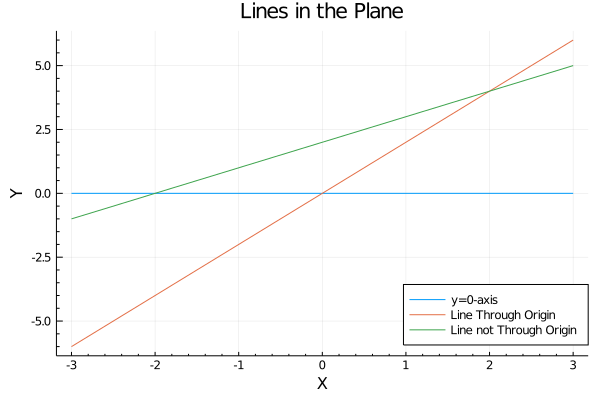
\includegraphics[width=0.6\textwidth]{Chap09VectorSpaceRnPart2/LinesInThePlane.png}
\caption{If a line does not pass through the origin, then it does not contain the origin, and hence it cannot be a subspace.}
\label{fig:LinesAreNotAlwaysSubspaces}
\end{figure}

\begin{tcolorbox}[title=\textbf{Easy First Test for Subspaces:}]
  Every subspace must contain the zero vector. Why? Suppose that $V \subset \real^n$ is a subspace and that $v\in V$. Then $0 \cdot v \in V$ because $V$ is closed under scalar times vector multiplication. But $0 \cdot v = 0$, the zero vector. Figure~\ref{fig:LinesAreNotAlwaysSubspaces} drives home the point that, even in $\real^2$, not all lines are subspaces. In fact, almost no lines are subspaces! It's a very special case when the $y$-intercept equals zero.
\end{tcolorbox}



\begin{example}
\label{ex:Subspace01}
Let $V\subset \real^2$ be the set of all points that lie on a line $y=mx+b$, that is
$$V:=\left\{ \begin{bmatrix} x \\ m x + b\end{bmatrix}~ \Big| ~ x \in \real \right\}. $$ Then $V$ is a subspace of $\real^2$ if, and only if, $b=0$, that is, the line must pass through the origin.
\end{example}




\textbf{Solution:} 
$V$ contains the zero vector if, and only, if the $y$-intercept is zero. But this means that $b=0$. Now, $0 \in V$ is a \textit{necessary condition}, but not a \textit{sufficient condition} for $V$ to be a subspace. So, let's check if $V$, with $b=0$ is closed under vector addition and scalar times vector multiplication. $V$ is then
$$V:=\left\{ \begin{bmatrix} x \\ m x\end{bmatrix}~ \Big| ~ x \in \real \right\}.$$
We take 
$$v_1 = \begin{bmatrix} x_1 \\ m x_1 \end{bmatrix}~\text{and}~v_2 = \begin{bmatrix} x_2 \\ m x_2 \end{bmatrix} $$
for $x_1$ and $x_2$ arbitrary real numbers. Then
$$v_1 + v_2= \begin{bmatrix} x_1 + x_2 \\ m x_1 + m x_2 \end{bmatrix}=\begin{bmatrix} x_1 + x_2 \\ m (x_1 + x_2) \end{bmatrix} \in V,$$
and hence $V$ is closed under vector addition. To be extra clear, we note that
$$v_1 + v_2= \begin{bmatrix} x \\ m x \end{bmatrix}, ~\text{for}~x=x_1 + x_2,$$
and that is why $v_1 + v_2 \in V.$\\

We now let $\alpha \in \real$ be arbitrary and check scalar times vector multiplication.
$$\alpha v_1= \alpha \begin{bmatrix} x_1  \\ m x_1  \end{bmatrix}=\begin{bmatrix} \alpha x_1 \\ \alpha m x_1 \end{bmatrix} = \begin{bmatrix} \alpha x_1 \\ m ( \alpha  x_1) \end{bmatrix} \in V,$$
and hence $V$ is closed under  scalar times vector multiplication. To be extra clear, we note that
$$\alpha v_1 = \begin{bmatrix} x \\ m x \end{bmatrix}, ~\text{for}~x=\alpha x_1,$$
and that is why $\alpha v_1 \in V.$\\

Suppose that $b\ne 0$. Can we show that $V$ is not a subspace without taking the shortcut of first checking that $V$ contains the zero vector? The answer is yes. Let's do vector addition with $b \neq 0$. Then 
$$v_1 = \begin{bmatrix} x_1 \\ m x_1 + b\end{bmatrix}~\text{and}~v_2 = \begin{bmatrix} x_2 \\ m x_2 +b\end{bmatrix} $$
and
$$v_1 + v_2= \begin{bmatrix} x_1 + x_2 \\ m x_1 + m x_2 + 2 b \end{bmatrix}=\begin{bmatrix} x_1 + x_2 \\ \left( m (x_1 + x_2) + b \right) + \boxed{b} \end{bmatrix} \not \in V.$$
We see that we cannot write
$$v_1 + v_2 = \begin{bmatrix} x \\ mx+b \end{bmatrix} $$
for some $x$ in $\real$, when $b \neq 0$, and that is why $V$ is not closed under vector addition. You can also check that it is not closed under scalar times vector multiplication, but for the purpose of showing a subset of $\real^n$ is not a subspace, you only need to violate ONE of the conditions.
\Qed

\begin{example}
\label{ex:Subspace02}
$V:=\real^n$ is a subspace of $\real^n$ and $W:=\{  0_{n \times 1} \} \subset \real^n$, the zero vector, is a subspace of $\real^n$
\end{example}

\textbf{Solution:} We'll let you apply the definition to $V$ and check that it is a subspace. $V$ is the largest subspace of $\real^n$, because it is all of $\real^n$, while $W$ is the smallest subspace of $\real^n$, since it consists only of the zero vector. Is $W$ really a subspace? Well, if we add any two vectors in $W$, we are adding $n \times 1$ zero vectors, and we'll get the $n \times 1$ zero vector. If we take any real number $\alpha \in \real$ and vector $w\in W$, then we are multiplying the $n \times 1$ zero vector by $\alpha$, and we get once again the $n \times 1$ zero vector. Hence, $W$ is closed under the operations of vector addition and scalar times vector multiplication, showing that it is a subspace. \Qed

\begin{example}
\label{ex:Subspace03}
$V:=\left\{ \begin{bmatrix} x_1 \\ 0 \\  x_1+ 4 x_2\end{bmatrix}~ \Big| ~ x_1, x_2 \in \real \right\}$ is a subspace of $\real^3$, while $W:=\left\{ \begin{bmatrix} x_1 \\ 5 \\ x_1+ 4 x_2 \end{bmatrix}~ \Big| ~ x_1, x_2 \in \real \right\}$ is a NOT subspace of $\real^3$. 
\end{example}

\textbf{Solution:} $W$ does not contain the zero vector and hence it cannot be a subspace. What about $V$? We write
$$v_1 = \begin{bmatrix} \overline{x}_1 \\ 0 \\ \overline{x}_1 + 4 \overline{x}_2\end{bmatrix}~\text{and}~v_2 = \begin{bmatrix} \doverline{x}_1 \\ 0 \\ \doverline{x}_1 + 4 \doverline{x}_2\end{bmatrix}. $$
Then, 
$$ v_1 + v_2 = \begin{bmatrix} \overline{x}_1 +  \doverline{x}_1 \\ 0 \\ \overline{x}_1 + 4 \overline{x}_2 +  \doverline{x}_1 + 4 \doverline{x}_2\end{bmatrix} = \begin{bmatrix} (\overline{x}_1 +  \doverline{x}_1) \\ 0 \\ (\overline{x}_1 + \doverline{x}_1) + 4  (\overline{x}_2 + \doverline{x}_2)\end{bmatrix}= \begin{bmatrix} x_1 \\ 0 \\  x_1+ 4 x_2\end{bmatrix}$$
for $x_1 = (\overline{x}_1 + \doverline{x}_1)$ and $x_2 = (\overline{x}_2 + \doverline{x}_2)$. Hence, $v_1 + v_2 \in V.$ \\

Working out $\alpha v_1 \in V$ for all $\alpha \in \real$ follows the same pattern. We conclude that $V$ is a subspace. \Qed
\vspace*{.5cm}

\subsection{(Optional Read:) A Broader View of Subspaces}
\label{sec:FunctionSpaces}

For some readers, this section may be very helpful and for others, it may be a total distraction. You have to decide for yourself!\\

The key property of vectors is that we know how to form linear combinations of them. Do we know other sets of ``things'' where we can add them up and get another element of the set and also multiply an element of the set by an arbitrary real number and obtain another element of the set? We submit that you know how to add a finite number of functions to produce another function, and you know how to multiply a function by a real number to define a new function! Hence, the set of all functions from the reals to the reals,
$$ X := \{ f:\real  \to \real \},$$
is closed under linear combinations and is a vector space. The set includes complicated functions such as $f(x) = x^3 \sin(e^x) - x^5$, radial basis functions $r(x)=e^{\frac{(x - x_c)^2}{s^2}},$ and simpler functions such as $g(x) = 1 + x$. \\

\begin{example} What is the zero vector in the vector space $X$?   
\end{example}

\textbf{Solution:} It would be the zero function, ${\rm zero}:\real \to \real$ by ${\rm zero}(x) = 0$ for all $x \in \real$. It is the only function satisfying ${\rm zero}(x) + f(x) = f(x)$ for all vectors (functions) in $X$.
\Qed\\

Can we define any interesting subsets of this vector space? And would they be subspaces of $X$? How about we consider the set of all polynomials with real coefficients? That is, 
$$P:=\{ p(x) \in X~|~ p(x) \text{ is a polynomial } \}.$$
$P$ is clearly a subset of $X$ because polynomials are special types of functions. Is it a subspace? Well, the sum of any two polynomials is a polynomial, and when we multiply a polynomial by a real number (that is, we multiply each of its coefficients by the same real number), we obtain another polynomial. Hence, $P$ is a subspace of $X$. \\

We could also define
$$ P_n:=\{ p(x) \in P~|~ \text{ the degree of }p(x) \text{ is less than or equal to }n \}.$$
Do we know specific vectors in $P_n$? Sure! How about 
$$ \{ 1(x), x, x^2, \ldots, x^n \},$$
where $1(x)$ here is denoting the constant function $1(x):=1=x^0$ for all $x\in \real$. Wait, those are vectors? They are vectors in the vector space $X$, the set of all functions from the reals to the reals: $v_k(x):=x^k$, $0 \le k \le n$ are perfectly good functions, called the monomials. Moreover, every polynomial consists of linear combinations of monomials!\\

Using notation that we introduce in the next section,
$$ P_n = \spanof{x^0, x, x^2, \ldots, x^n},$$
which means that every polynomial of degree less than or equal to $n$ can be written as a linear combination of the monomials from $x^0$ to $x^n$. It's also clear that if we remove any elements from this set, then there would be polynomials of degree less than or equal to $n$ that we could not generate. Hence, this set is the smallest one that can generate all polynomials of degree $n$ or less.\\


Using ideas from Chapter~\ref{sec:OrthogonalProjection}, we could find a polynomial of a fixed degree that is the best approximation\footnote{There are some technicalities that we are skipping. The function and its square would have to be Riemann integrable (for us engineers, Lebesgue integrable for mathematicians), and we would have to do the best fit over a bounded interval $[a, b]\subset \real$, $a < b$.} of a general function in $X$. That is a useful idea and we have explored a special case of it in homework and in Project 2. 



\begin{example} Is the set $V:=\{ p(x) \in P~|~ \text{ the degree of }p(x) \text{ is exactly equal to }n \}$ a subspace, for $n\ge 1$?     
\end{example}

\textbf{Solution:} No, because the zero vector does not have degree $n$ and hence is not an element of the set, $V$. Another way to see it is that if we define $p_1(x) = 2 +  3 x^n$ and $p_2(x)= x^n$, then $p_1(x), p_2(x) \in V$, but their linear combination $p_1(x) - 3 p_2(x) \not \in V$.

\Qed

\section{Three Sources of Subspaces in $\real^n$: Matrix Null Space, Span of a set of Vectors, and Column Span of a Matrix}

\begin{tcolorbox}[sharp corners, colback=green!30, colframe=green!80!blue, title=\textbf{\Large Null Space of a Matrix}]
For an $n \times m$ matrix $A$, its \textbf{null space} is $$\nullspace(A):=\{x \in \real^m~|~ A x = 0_{n \times 1} \},$$
the set of all solutions (that is, vectors) that result in $Ax$ being the zero vector or the ``null vector''. \\

\textbf{Remark:} $Ax=0$ has a unique solution if, and only if, $\nullspace(A)=\{ 0_{m \times 1} \}$, the zero vector in $\real^m$. If $Ax=b$ has a solution and $\nullspace(A) \neq \{ 0_{m \times 1} \}$, then the equation has an infinite number of solutions. We will later find the solution with minimum norm.

\end{tcolorbox}

\vspace*{.2cm}

\begin{example}
\label{ex:NullSpaceComputitingIt} 
Compute the null space of $A= \left[\begin{array}{ccc} 1 & 3 & 0\\
0 & 4 &  1\end{array}\right]$.

 \end{example}

\textbf{Solution:} We note that $A$ is a $2 \times 3$ matrix. Hence, its null space is $$\nullspace(A):= \{ x \in \real^3~|~ A x = 0_{2 \times 1} \} \subset \real^3. $$
Moreover, 
\begin{align*}
  A x &= 0_{2 \times 1} \iff \left[\begin{array}{rrr}1 & 3  & 0 \\ 0 & 4 & 1 \end{array}\right]\left[\begin{array}{r} x_1 \\ x_2 \\ x_3\end{array}\right] = 0_{2 \times 1} \iff \begin{cases}
    \begin{aligned}
     x_1 + 3x_2 + 0 x_3 &=0 \\
     0 x_1 +4x_2 + 1 x_3&= 0
    \end{aligned} \end{cases} \iff \begin{cases}
    \begin{aligned}
     x_1&=-3x_2 \\
     x_3&= -4x_2.
    \end{aligned} \end{cases} 
\end{align*} 
Hence, $$x \in \nullspace(A) \iff  
x = \left[\begin{array}{r} -3x_2 \\ x_2 \\ -4x_2 \end{array}\right] = \left\{  x_2 \left[\begin{array}{r} -3 \\ 1\\ -4 \end{array}\right] ~ \Big| ~ x_2 \in \real \right\} = \left\{  \alpha \left[\begin{array}{r} -3 \\ 1\\ -4 \end{array}\right] ~ \Big| ~ \alpha \in \real \right\},$$
where we replaced $x_2$ with $\alpha$ for purely cosmetic reasons, meaning that we did it to emphasize that $x_2$ was really just an arbitrary scalar.
\Qed \\

\textbf{Remark:} Anticipating the next definition, we can express the null space of $A$ as 
$$\text{null}(A) = \spanof{\left[\begin{array}{r} -3 \\ 1 \\ -4 \end{array}\right]}:=\left\{  \alpha \left[\begin{array}{r} -3 \\ 1\\ -4 \end{array}\right] ~ \Big| ~ \alpha \in \real \right\}.$$

\textbf{Remark:} Additional worked examples are in Chapter \ref{chap:matrixFacts}, Example \ref{ex:Subspace04}.

\vspace*{.2cm}

\begin{example}
\label{ex:NullSpaceIsSubSpace} 
For an $n \times m$ matrix $A$, show that $\nullspace(A)$ is a subspace of $\real^m$.
 \end{example}

\textbf{Solution:} Suppose $v_1, v_2 \in \nullspace(A)$, so that $A v_1 = A v_2 =  0_{n \times 1}$. We need to show that for all real numbers $\alpha$ and $\beta$, 
\begin{equation}
    \alpha v_1 + \beta v_2  \in \nullspace(A)~~\text{(closed under linear combinations)}.
\end{equation}
But, $A \left(   \alpha v_1 + \beta v_2 \right) =  \alpha  A v_1 + \beta A v_2 = \alpha ~0_{n \times 1} + \beta ~0_{n \times 1} = 0_{n \times 1}$, and thus 
$ \alpha v_1 + \beta v_2 \in \nullspace(A)$.
\Qed


\vspace*{.2cm}

\begin{tcolorbox}[sharp corners, colback=green!30, colframe=green!80!blue, title=\textbf{\Large Span of a Set of Vectors}]
Suppose that $S \subset \real^n$, then $S$ is a set of vectors. The set of all possible linear combinations of elements of $S$ is called the span of $S$,
$$\spanof{S}:=\{ \text{all possible linear combinations of elements of}~S \}. $$

\textbf{It follows that $\spanof{S}$ is a subspace of $\real^n$ because, by definition, it is closed under linear combinations.} This is true for any subset $S \subset \real^n$.\\

\textcolor{red}{\bf What is the span good for?} The span operation is how one takes an arbitrary set of vectors and generates a subspace from it. If $S$ is a set, $\spanof{S}$ is the smallest subspace that contains all of the elements of the set $S$. Shortly, we'll find a different set, $\widetilde S$, such that $\spanof{S}=\spanof{\widetilde S}$ AND $\widetilde S$ is a ``nicer'' set of vectors.
\end{tcolorbox}

\vspace*{.2cm}

If a set $S$ is already known to be a subspace of $\real^n$, then taking its span does not add any new vectors because a subspace is closed under linear combinations. Hence, $S \subset \real^n$ and $S$ a subspace $\implies \spanof{S}=S.$ When $S$ is not a subspace, then there is at least one linear combination of elements of $S$ that is not in $S$ itself. In this case, the span is a bigger set, meaning that $S\subset \spanof{S}$ and $S \neq \spanof{S}$. \\

\begin{example}
\label{ex:Span01} Consider the vector space $\real^3$ and two vectors $e_1$ and $e_2$, where for $k=1,2$, $e_k$ has a one in the $k$-th entry and zeros elsewhere. In other words, $e_1$ and $e_2$ are the first and second columns of $I_3$, the $ 3\times 3$ identity matrix. Compute $\spanof{e_1+e_3, e_2+e_3}$.
 \end{example}

\textbf{Solution:} We have $S=\{ e_1+e_3, e_2+e_3\}.$ The set $\{ e_1+e_3, e_2+e_3\}$ is not a subspace because the vector $e_1 -e_2 = (e_1+e_3) - (e_1 + e_3) \not \in S$. 
\begin{align*}
    \spanof{S}&:=\{ \text{all possible linear combinations of elements of}~S \} \\
    &= \left\{ \alpha_1 (e_1+ e_3) + \alpha _2 (e_2+e_3)~\Big|~ \alpha_1\in \real, \alpha_2 \in \real \right\} \\
    &=  \left\{ \alpha_1 \left[\begin{array}{c}  1\\ 0 \\ 1 \end{array} \right] + \alpha_2 \left[\begin{array}{c}  0 \\ 1 \\ 1 \end{array} \right]~\Big|~ \alpha_1 \in \real, \alpha_2 \in \real \right\} \\
    & =\left\{  \left[\begin{array}{c}  \alpha_1\\ \alpha_2 \\ \alpha_1 + \alpha_2 \end{array} \right] ~\Big|~ \alpha_1\in \real, \alpha_2 \in \real \right\} \\
    & =\left\{  \left[\begin{array}{c}  x\\ y\\ x+y \end{array} \right] ~\Big|~ x\in \real, y \in \real \right\} \\
      & =\left\{  \left[\begin{array}{c}  x\\ y\\ z \end{array} \right] ~\Big|~ z = x+y, x\in \real, y \in \real \right\}. 
\end{align*}
Hence,  $\spanof{e_1+e_3, e_2+e_3}$ is the plane given by $z = x+y$ in $\real^3$. \Qed\\

For this very simple and very special case, we could ``recognize'' what the span of the set of vectors turned out to be and name it. More generally, we cannot ``recognize'' what the span looks like. We simply use it as convenient notation when we want to work with the linear combinations associated with a set of vectors and not just the vectors themselves. 


\begin{figure}[htb]%
\centering
\subfloat[]{%
    \label{fig:NullSpaceA}%
\centering
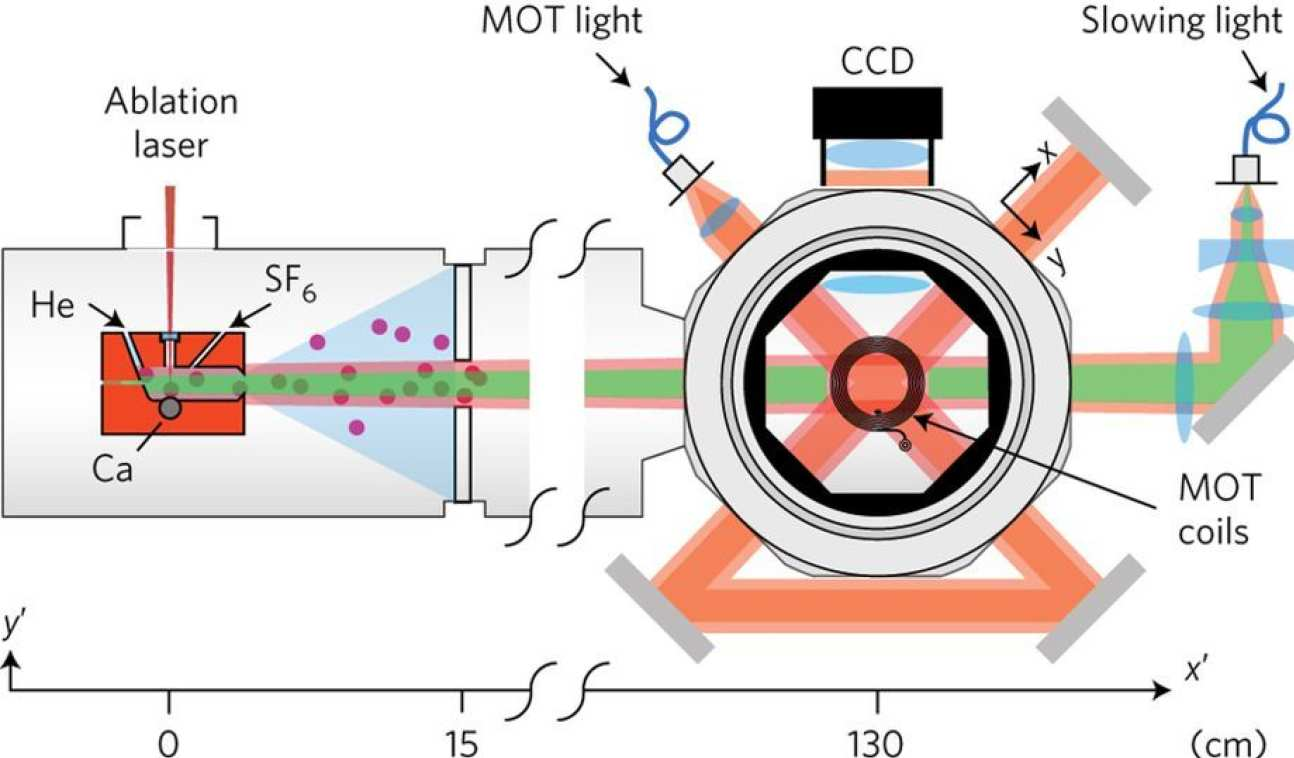
\includegraphics[width=0.4\textwidth]{Chap09VectorSpaceRnPart2/ImperialCollegeLondon_chamber--tojpeg_1572173408083_x2.jpg}
}
\hspace{5pt}%
\subfloat[]{%
    \label{fig:NullSpaceB}%
	\centering
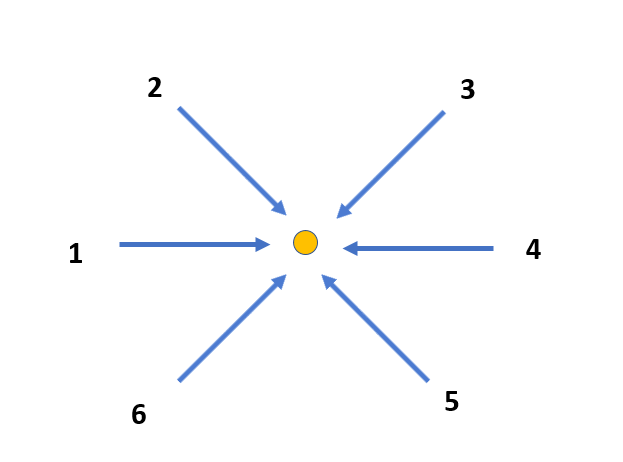
\includegraphics[width=0.40\textwidth]{Chap09VectorSpaceRnPart2/LaserCoolingSketch.png}}%
\caption[]{Where do null spaces come from ? (a) A chamber to cool molecules to near absolute zero, courtesy of Imperial College of London. The laser beams cool the center object by pushing on it to reduce its ``vibrational energy''. You can think of it as ``clamping the molecule in place''. (b) A toy example we use to illustrate null spaces. Arrows 2, 3, 5, and 6 are at 45$^o$.}
    \label{fig:NullSpace}
\end{figure}


\begin{example}
\label{ex:NullSpaceLaserCooling} \textbf{(Combining null space, span, and physical intuition)}
For the image in Fig.~\ref{fig:NullSpace}-(b), we imagine the laser beams as applying forces to the center molecule. Labeling the forces as $F_1$ through $F_6$ and balancing their $x$ and $y$ components to achieve an equilibrium results in 
\begin{equation}
\label{eq:CoolingMolecules}
    \underbrace{\left[\begin{array}{rrrrrr}  1 & \frac{\sqrt{2}}{2} & -\frac{\sqrt{2}}{2} & -1 & -\frac{\sqrt{2}}{2} & \frac{\sqrt{2}}{2} \bigskip \\
     0& -\frac{\sqrt{2}}{2} & -\frac{\sqrt{2}}{2} & 0 & \frac{\sqrt{2}}{2} & \frac{\sqrt{2}}{2}\end{array} \right]}_{A} \underbrace{\left[\begin{array}{c} F_1\\F_2 \\  F_3\\F_4 \\ F_5\\F_6 \\ \end{array} \right]}_{x} = \left[\begin{array}{c}  0\\ 0  \end{array} \right].
\end{equation}
Compute the null space of $A$ and interpret it!
 \end{example}

\textbf{Solution:} Newton's Laws tell us that for a particle to be in equilibrium, the forces acting on it must ``balance out'', which is ``physics-speak'' for saying that when you treat the forces as vectors in $\real^2$, their vector sum must add up to zero. This can also be interpreted as the sum of the forces in the $x$-direction must be zero and the same for the sum in the $y$-direction. This vector sum has been done for you in Equation \eqref{eq:CoolingMolecules}. The purpose of the problem is to understand that equilibrium problems like the one posed in the example correspond to null spaces of a matrix.\\

\textbf{Pure mathematical computation of the null space:} The matrix $A$ has two rows and six columns. A non-zero vector in the null space gives a non-trivial linear combination of the columns of $A$ that add up to the zero vector. We claim that there are four linearly independent vectors in the null space. Let's compute them! \\

The first two columns of $A$ are linearly independent; indeed the matrix 
$$\underbrace{\left[\begin{array}{rr}  1 & \frac{\sqrt{2}}{2} \bigskip \\ 0 & -\frac{\sqrt{2}}{2} \end{array} \right]}_{\overline{A}}$$
is triangular and has non-zero entries on its diagonal. We can use the linear independence of these two columns  to express each of the remaining four columns as linear combinations of the first two.\\

We write 
$$\left[ \begin{array}{rrrr}  b_1 & b_2 & b_3 & b_4 \end{array} \right] := \left[\begin{array}{rrrr}  -\frac{\sqrt{2}}{2} & -1 & -\frac{\sqrt{2}}{2} & \frac{\sqrt{2}}{2} \bigskip \\
     -\frac{\sqrt{2}}{2} & 0 & \frac{\sqrt{2}}{2} & \frac{\sqrt{2}}{2} \end{array} \right],$$
      so that the vectors $b_i$, $1 \le i \le 4$ are the remaining columns of $A$. We set up the equations
      $$\underbrace{\left[\begin{array}{rr}  1 & \frac{\sqrt{2}}{2} \bigskip \\ 0 & -\frac{\sqrt{2}}{2} \end{array} \right]}_{\overline{A}} \begin{bmatrix} \alpha_{i,1} \\ \\ \alpha_{i,2}  \end{bmatrix} = b_i,$$
     and note that because $\overline{A}$ is invertible, each of the equations has a unique solution. After slightly rearranging the above we have 
     $$  \alpha_{i,1} \left[\begin{array}{r}  1\\ 0 \end{array} \right] + \alpha_{i,2} \left[\begin{array}{r}  \frac{\sqrt{2}}{2}\\ -\frac{\sqrt{2}}{2} \end{array} \right] - b_i = 0_{2 \times 1}.$$
     It follows that the four vectors 
     $$ \left\{ v_1 = \left[ \begin{array}{r} \alpha_{1,1}  \\ \alpha_{1,2} \\ -1 ~~\\ 0 ~~\\ 0 ~~\\ 0 ~~\end{array} \right], v_2 = \left[ \begin{array}{r} \alpha_{2,1}  \\ \alpha_{2,2} \\ 0 ~~\\ -1~~\\ 0~~\\ 0~~\end{array} \right], v_3 = \left[ \begin{array}{r} \alpha_{3,1}  \\ \alpha_{3,2} \\ 0 ~~\\ 0~~\\ -1~~\\ 0~~\end{array} \right], v_4 =  \left[ \begin{array}{r} \alpha_{4,1}  \\ \alpha_{4,2} \\ 0~~ \\ 0~~\\ 0~~\\ -1~~\end{array} \right]  \right\}$$
     are in the null space of $A$ because 
     
     $$\begin{aligned} A v_i & =  \left[\begin{array}{rrrrrr}  1 & \frac{\sqrt{2}}{2} & -\frac{\sqrt{2}}{2} & -1 & -\frac{\sqrt{2}}{2} & \frac{\sqrt{2}}{2} \bigskip \\
     0& -\frac{\sqrt{2}}{2} & -\frac{\sqrt{2}}{2} & 0 & \frac{\sqrt{2}}{2} & \frac{\sqrt{2}}{2}\end{array} \right] v_i\\
     & =\alpha_{i,1} \left[\begin{array}{r}  1\\ 0 \end{array} \right] + \alpha_{i,2} \left[\begin{array}{r}  \frac{\sqrt{2}}{2}\\ -\frac{\sqrt{2}}{2} \end{array} \right] - b_i \\
     & = 0_{2 \times 1}. \end{aligned}  $$
     We'll leave it to the reader to check that the four vectors $\{v_1, v_2, v_3, v_4\}$ are linearly independent. Once you note that the last four entries of $\{v_1, v_2, v_3, v_4 \}$ consist of zeros and negative ones, showing independence is very quick!\\
     
Could there be more than four linearly independent vectors in the null space of $A$? We'll prove in Chapter~\ref{sec:RankNullity} that four is the magic number and that this follows from the much easier observation that $A$ has two linearly independent rows and six columns! Hence, 
$$ \nullspace(A) = \spanof{v_1, v_2, v_3, v_4}.$$
 
 \vspace*{.2cm}    

\textbf{We next give a completely different method and claim that we can ``see'' the null space from the diagram.} If we increase $F_1$ and $F_4$ by the same amount, then they cancel in both the $x$ and $y$ directions. If we increase  $F_2$ and $F_5$ by the same amount, then they cancel.  If we increase $F_3$ and $F_6$ by the same amount, then they cancel. And finally, if we increase  $F_2$ and $F_6$ by the same amount, their $y$-components cancel but, not their $x$-components, so we need to offset that by $F_4$. Ta da! Pretty cool, right? This gives
\begin{equation}
    \label{eq:HandComputeNullSpace}
    \nullspace(A)={\rm span}\left\{ \left[\begin{array}{c} 1\\0 \\  0\\1 \\ 0\\0 \\ \end{array} \right],
\left[\begin{array}{c} 0\\1\\  0\\0 \\ 1\\0 \\ \end{array} \right],
\left[\begin{array}{c} 0\\0 \\  1\\0 \\ 0\\1 \\ \end{array} \right],
\left[\begin{array}{r} 0\\1 \\  0\\ \sqrt{2} \\ 0\\1 \\ \end{array} \right]
    \right\},
\end{equation}
where
$$\left[\begin{array}{c} 1\\0 \\  0\\1 \\ 0\\0 \\ \end{array} \right] \leftrightarrow F_1 \text{ and } F_4 \text{ balancing one another, }
\left[\begin{array}{c} 0\\1\\  0\\0 \\ 1\\0 \\ \end{array} \right] \leftrightarrow F_2 \text{ and } F_5 \text{ balancing one another }$$

$$\left[\begin{array}{c} 0\\0 \\  1\\0 \\ 0\\1 \\ \end{array} \right] \leftrightarrow F_3 \text{ and } F_6 \text{ balancing one another, }
\left[\begin{array}{r} 0\\1 \\  0\\ \sqrt{2} \\ 0\\1 \\ \end{array} \right] \leftrightarrow F_2, \sqrt{2} F_4 \text{ and } F_6 \text{ balancing.}~~~~~$$
The null space is then all linear combinations of forces that result in the particle being in equilibrium. This same principle was used to analyze the truss-bridge example in Fig.~\ref{fig:TrussBridgeCartoons}.\\

\begin{tcolorbox}[title={\bf Statics Problems and Null Spaces}]
 When you take a Statics \& Dynamics course, all of the statics problems involve computing forces that lie in null spaces of matrices, where the matrices represent the (vector) sum of the forces (and possibly torques) being zero. 
\end{tcolorbox}

\vspace*{.2cm}


\textbf{Question:} Are we missing the linear combination of $F_3$, $F_5$ and $F_1$ given by
$$\left[\begin{array}{r} \sqrt{2} \\0 \\  1\\ 0\\ 1\\0 \\ \end{array} \right] ?$$ Analogously to how  $F_2$, $F_6$, and $F_4$ work together, this vector will also result in a zero net change to the force equilibrium, won't it? The answer is a resounding yes, but it is already included in the above span, because
$$\left[\begin{array}{r} \sqrt{2} \\0 \\  1\\ 0\\ 1\\0 \\ \end{array} \right] =\sqrt{2}
 \left[\begin{array}{c} 1\\0 \\  0\\1 \\ 0\\0 \\ \end{array} \right] +
\left[\begin{array}{c} 0\\1\\  0\\0 \\ 1\\0 \\ \end{array} \right] +
\left[\begin{array}{c} 0\\0 \\  1\\0 \\ 0\\1 \\ \end{array} \right]-
\left[\begin{array}{r} 0\\1 \\  0\\ \sqrt{2} \\ 0\\1 \\ \end{array} \right].$$

\textbf{Question:} Is it a problem that the four vectors we found in our mathematical calculation are different than the four vectors we found using physical reasoning based on force balancing? The answer is no. We invite you to go to Julia and check that the two spans are the same, which you can do by writing the vectors in one span as linear combinations of the vectors in the other span. In Chapter~\ref{sec:BasisCoordinatesDimension}, we will introduce the notion of a \textit{basis for a subspace}. Our two methods of computing the null space of $A$ have produced two different sets of basis vectors. Is one better than the other? No. Do you like one more than the other? Probably! Some of you will like the physical reasoning and some will be hard-core math types. The world needs all types! \\


Hopefully, this example helps to clarify  linear combinations, span, and null space.
\Qed

\vspace*{0.2cm}

\begin{example}
\label{ex:SpanCircle} Let $S$ be the unit circle in $\real^2$. Compute $\spanof{S}$. 
 \end{example}

\textbf{Solution:} We have that $S:=\{(x_1,x_2)~| (x_1)^2 + (x_2)^2=1  \} \subset \real^2$, which has an infinite number of elements. Hence, computing its span must be super tricky, right? Not really. We note that $e_1$ and $e_2$ are both elements of $S$ because $e_1$ corresponds to $x_1=1$ and $x_2=0$, while $e_2$ corresponds to $x_1=0$ and $x_2=1$. Hence,
$$\spanof{e_1,e_2} \subset \spanof{S}.  $$
But we know that $\spanof{e_1,e_2} = \real^2$ and $\spanof{S} \subset \real^2$, where the last statement is true because every element of $S$ is in $\real^2$ and a linear combination of vectors in $\real^2$ gives another vector in $\real^2$. Therefore,
$$ \real^2 = \spanof{e_1,e_2} \subset \spanof{S}  \subset \real^2,$$
which shows that $\spanof{S}  = \real^2$.
\Qed



% \begin{example}
% \label{ex:SpanCircleB} Let $S$ be the unit circle in $\real^2$. Show that $S$ is linearly dependent. 
%  \end{example}

% \textbf{Solution:} We'll give a couple solutions. First, we note that both $v_1:=e_1$ and $v_2:=-e_1$ are in $S$. But the set $\{ v_1, v_2\}$ is linearly dependent because $v_1 + v_2=0$. Here's a second solution. We note that $v_1:=e_1$, $v_2:=e_2$, and $v_3:=\frac{\sqrt{2}}{2} e_1 + \frac{\sqrt{2}}{2} e_2 $ are all in $S$. But the set $\{v_1, v_2, v_3  \}$ is linearly dependent because $\frac{\sqrt{2}}{2} v_1 + \frac{\sqrt{2}}{2} v_2 -v_3 = 0$.

% \Qed

% \begin{example}
% \label{ex:SpanLine} Let $S$ be the line in $\real^3$ defined by
% $$S:=\{ (x_1,x_2,x_3)~|~ x_3 = x_2-x_1 +1 \}. $$
% Compute $\spanof{S}$. 
%  \end{example}

% \textbf{Solution:} Easy calculations show that $\{ e_3, e_1, -e_2\} \subset S$. Indeed, taking $x_1=x_2=0$ and $x_3=1$ gives a point on the line; taking $x_1=1$, $x_2=0$ and $x_3=0$ gives another point on the line, and finally,  taking $x_1=0$, $x_2=-1$ and $x_3=0$ gives still another point on the line. Hence, we have that
% $$\spanof{e_3, e_1,-e_2} \subset \spanof{S}.  $$
% But we know that $\spanof{e_3, e_1, -e_2} = \real^3$ and $\spanof{S} \subset \real^3$, where the last statement is true because every element of $S$ is in $\real^2$ and a linear combination of vectors in $\real^3$ gives another vector in $\real^3$. Therefore,
% $$ \real^3 = \spanof{e_3, e_1, -e_2} \subset \spanof{S}  \subset \real^3,$$
% which shows that $\spanof{S}  = \real^3$.
% \Qed



\begin{tcolorbox}[sharp corners, colback=green!30, colframe=green!80!blue, title=\textbf{\Large Column Span of a Matrix}]
Let $A$ be an $n \times m$ matrix. Then its columns are vectors in $\real^n$. Their span is called the \textbf{column span of} ${\bf A}$.
$$\colspanof{A}:=\spanof{a^{\rm col}_1, \ldots, a^{\rm col}_m }. $$

We saw in Chapter~\ref{sec:UniquenessSolutions} that $Ax=b$ has a solution if, and only if, $b$ is a linear combination of the columns of $A$. A more elegant way to write this is\newline
\centerline{\bf ${\bf Ax=b}$ has a solution if, and only if, ${\bf b \in \colspanof{A}}$}. 
\end{tcolorbox}

\vspace*{.2cm}
\begin{example}
\label{ex:ColSpan01} Suppose $A=\left[\begin{array}{rrr}  3 & 2\\ 1 & -2 \\ -1 & 1 \end{array} \right]$ and $b=\left[\begin{array}{r} 0 \\ -8 \\ 5 \end{array} \right]$. Does $Ax=b$ have a solution? 
 \end{example}

\textbf{Solution:}  This is identical to the problems we solved in Chapter~\ref{sec:AttractiveTestLinearCombination}. We check that 
$$b=-2 a^{\rm col}_1 +  3 a^{\rm col}_2 \in \spanof{a^{\rm col}_1, a^{\rm col}_2},$$
and hence $b$ is in the column span of $A$, and the system of linear equations has a solution, namely,
$$x=\left[\begin{array}{r} -2 \\3 \end{array} \right] $$
is a solution!\Qed


\vspace*{.2cm}

\textcolor{red}{\bf Here is an intriguing example.}

\begin{example}
\label{ex:IlluminatingOrthonormalVectors}
Consider the matrices 
\begin{equation}
A:=\left[
\begin{array}{rrr}
0.8399 & -1.1136 & -0.7449 \\
-0.8898 & 0.9555 & -0.1578 \\
0.0069 & 0.8307 & -0.8218 \\
-1.1286 & 2.0774 & -0.2728 \\
-0.0115 & -0.2561 & 0.1850 \\
\end{array}
\right]_{5 \times 3} \text{ and  } Q:=
\left[
\begin{array}{rrr}
0.5046 & 0.1296 & -0.7328 \\
-0.5345 & -0.3516 & -0.6560 \\
0.0041 & 0.8038 & -0.1712 \\
-0.6780 & 0.3812 & -0.0287 \\
-0.0069 & -0.2612 & -0.0492 \\
\end{array}
\right]_{5 \times 3}.
\end{equation}
Is the vector 
\begin{equation}
b:=\left[
\begin{array}{r}
-0.4524 \\
-0.9162 \\
0.8603 \\
0.4963 \\
-0.3618 \\
\end{array}
\right]
\end{equation}
a linear combination of the columns of $A$? In other words, is $b \in \colspanof{A}$?

\end{example}

{\bf Solution:} The matrix $Q$ has been constructed using methods covered in Chapter~\ref{sec:OrthognalStuff} to satisfy $Q^\top Q = I_3$ and 
$$ \colspanof{A} = \colspanof{Q};$$
hence, 
$$b \in \colspanof{A} \iff b \in \colspanof{Q}. $$
\textcolor{red}{\bf For matrices that satisfy $Q^\top \cdot Q = I_n$ for some $n$, it must be easy to check $b \in \colspanof{Q}$, right?} Indeed, we'll later show that
$$  b \in \colspanof{Q} \iff b =  Q \alpha, \text{ for } \alpha := Q^\top b.$$
In Julia, we verify these conditions, and we're done. We have checked that $Ax = b$ has a solution.
\Qed

\vspace{.5cm}
 
\textbf{(Optional Read) Remark:} \textcolor{blue}{\bf Is the above method (which we will study in more detail later), better than our previous method with LDLT (recall Chapter~\ref{sec:AttractiveTestLinearCombination})? It can be faster in Julia because it involves fewer computations.} In Example~\ref{ex:IlluminatingOrthonormalVectors}, once we had $Q$, we needed to perform two matrix times vector multiplications, namely
$$ 
\alpha:=Q^\top b = \left[
\begin{array}{rrrrr}
0.5046 & -0.5345 & 0.0041 & -0.6780 & -0.0069 \\
0.1296 & -0.3516 & 0.8038 & 0.3812 & -0.2612 \\
-0.7328 & -0.6560 & -0.1712 & -0.0287 & -0.0492 \\
\end{array}
\right]_{3 \times 5} \left[
\begin{array}{r}
-0.4524 \\
-0.9162 \\
0.8603 \\
0.4963 \\
-0.3618 \\
\end{array}
\right]=  \left[
\begin{array}{r}
-0.0690 \\
1.2386 \\
0.7889 \\
\end{array}
\right] 
$$
and 
$$
Q \alpha = \left[
\begin{array}{rrr}
0.5046 & 0.1296 & -0.7328 \\
-0.5345 & -0.3516 & -0.6560 \\
0.0041 & 0.8038 & -0.1712 \\
-0.6780 & 0.3812 & -0.0287 \\
-0.0069 & -0.2612 & -0.0492 \\
\end{array}
\right]_{5 \times 3}
\left[
\begin{array}{r}
-0.0690 \\
1.2386 \\
0.7889 \\
\end{array}
\right] = \left[
\begin{array}{r}
-0.4524 \\
-0.9162 \\
0.8603 \\
0.4963 \\
-0.3618 \\
\end{array}
\right],
$$
and then verify $Q \alpha - b = 0_{5 \times 1}$. We will learn shortly that $Q$ comes from an algorithm that is similar to a matrix factorization. With LDLT, we would have to perform two matrix products, namely $A^\top \cdot A$ and $A_e^\top \cdot A_e$ for $A_e:=[A~~b]$, and two matrix factorizations. A product of a matrix and a vector is generally faster to compute than a matrix times another matrix, and all things being equal, computing one ``factorization'' is faster than computing two of them. While this is not a rigorous analysis, it gives you a sense that it may be worthwhile to learn about matrices that satisfy $Q^\top \cdot Q = I_n$!

\begin{example}
\label{ex:AnotherSubspaceExample}  Check if the following subsets of $\real^3$ are also subspaces of $\real^3$.

\begin{enumerate}
\renewcommand{\labelenumi}{(\alph{enumi})}
\setlength{\itemsep}{.2cm}
\item $S_1=\{ x\in \real^3~|~ \left[\begin{array}{ccc} 2.0 &  -1.0 & 11.0\end{array}\right] x = 1.0 \}$ 

\item $S_2=\{ x\in \real^3~|~ \left[\begin{array}{ccc} 2.0 &  -1.0 & 11.0 \end{array}\right] x = 0.0 \}$


\item $S_3 = \spanof{S_1}$
\end{enumerate}
 \end{example}

\textbf{Solution:} 

\begin{enumerate}
\renewcommand{\labelenumi}{(\alph{enumi})}
\setlength{\itemsep}{.2cm}
\item The zero vector is not contained in $S_1$. According to the fact that every subspace must contain the zero vector, $S_1$ is not a subspace of $\real^3$.

\item $S_2$ is the null space of the $1 \times 3$ matrix $A:= \left[\begin{array}{ccc} 2.0 &  -1.0 & 11.0\end{array}\right]$, and hence is a subspace.


\item The span of any subset of $\real^n$ is always a subspace. This is a sufficient answer. 
\end{enumerate}
\Qed

\begin{example}
\label{ex:AnotherSpanExample}  For each example, find linearly independent vectors that span the given subspace:

\begin{enumerate}
\renewcommand{\labelenumi}{(\alph{enumi})}
\setlength{\itemsep}{.2cm}

\item $V_1$ is defined to be the span of the columns of $B_1$, where 
$$B_1=\left[\begin{array}{cc} 1 & 2\\
1 & 3 \\
1 & 4\end{array}\right]. $$ 

\item $V_2$ is defined to be the span of the columns of $B_2$, where 
$$B_2=\left[\begin{array}{cc} 1 & 2\\
1 & 2 \\
1 & 2\end{array}\right]. $$ 


\item $V_3:=\spanof{S_3}$, where $S_3=\{ x\in \real^2~|~ (x_1)^2 + (x_2)^2 = 1\}$ (do not miss that $V_3 \subset \real^2$). 

\item $V_4:= \spanof{S_4}$, where $S_4=\{ x\in \real^4~|~ x_1+ 3x_2 + x_3 + 3 x_4 = 3\}$ (do not miss that $V_4 \subset \real^4$). 


\end{enumerate}


\end{example}

\textbf{Solutions:}  The first two problems are easy because you are directly given a finite set of vectors that span the subspace in question. The only issue is whether they are linearly independent or not. The last two problems are more challenging! Let's get to work.

\begin{enumerate}
\renewcommand{\labelenumi}{(\alph{enumi})}
\setlength{\itemsep}{.1cm}

\item $V_1 :=  \spanof{ \underbrace{\left[\begin{array}{c} 1 \\1  \\ 1 \end{array}\right] }_{v_1}, \underbrace{ \left[\begin{array}{c}  2\\ 3 \\ 4\end{array}\right] }_{v_2} }.$ Hence, we already know vectors that span $V_1$. We need to check if the given vectors are linearly independent or not. If not, we'll throw away dependent vectors. \\

We quickly check that $\alpha_1 v_1 + \alpha_2 v_2 = 0_{3 \times 1}$
if, and only if, $\alpha_1 = \alpha_2 = 0$. Thus the columns of $B_1$ are linearly independent and they span the subspace $V_1$.

\item This time, $V_2 := \spanof{ \underbrace{\left[\begin{array}{c} 1 \\ 1  \\
1 \end{array}\right]}_{v_1}, \underbrace{ \left[\begin{array}{c}  2\\  2 \\
 2\end{array}\right] }_{v_2} }.$ We observe that $2 v_1 - v_2 = 0_{3 \times 1}$ and thus they are linearly dependent. Because each vector is non-zero, either one alone is linearly independent and hence we can choose either one as the linearly independent vector. For example,
\begin{itemize}
    \item $V_2 = \spanof{\underbrace{\left[\begin{array}{c} 1 \\
1  \\
1 \end{array}\right]}_{v_1} },$ or

\item $V_2 = \spanof{\underbrace{\left[\begin{array}{c}  2\\
 2 \\  2\end{array}\right]}_{v_2} }.$

 \item We could also write $V_2 = \spanof{ \left[\begin{array}{c}  11\\
11 \\ 11\end{array} \right] } $ because any non-zero multiple of $v_1$ is also a valid solution.

\end{itemize}



\item This problem is quite different from the previous two because we are not given an explicit finite set of vectors that span the subspace. Instead, we are given an implicit description of a set and then we are asked to compute the span of that set of vectors. This is more common in applications.  \\

Before attacking the problem, it's good to establish:\\

\textbf{Lemma}. If $A \subset B \subset \real^n$, then $ \spanof{A} \subset \spanof{B} \subset \spanof{ \real^n} = \real^n$. \\

\textbf{Proof:} If $v \in \spanof{A}$, then $v = \sum_{i=1}^Kc_i\cdot v_i$ for some constants $c_i \in \real$ and vectors $ v_i\in A $. But because $A \subset B$, we have that  $ v_i\in B $ for all $1 \le i \le K$ and hence $\sum_{i=1}^Kc_i\cdot v_i \in \spanof{B}.$ Therefore, $v \in \spanof{A} \implies v \in \spanof{B}$, which means that $ \spanof{A} \subset \spanof{B}$. The same reasoning can be applied to $B \subset \real^n$. Finally, why is $\spanof{ \real^n} = \real^n$? One way to look at it: $\real^n$ is (already) a vector space and is thus closed under linear combinations. Hence, the span operation does not create any new vectors. \Qed  \\

Let's now find some vectors in $S_3$. We note that $v_1:=\left[\begin{array}{c} 1 \\ 0 \end{array}\right] \in S_3$ and $v_2:=\left[\begin{array}{c} 0 \\ 1 \end{array}\right] \in S_3$. Hence, applying the Lemma, we have that 
$$ \{ v_1, v_2 \} \subset  S_3 \subset \real^2 \implies \spanof{ v_1, v_2 } \subset \spanof{S_3} \subset \spanof{\real^2} = \real^2.$$ 
Next, we note that
 $$ \spanof{ v_1, v_2 } = \spanof{\left[\begin{array}{c} 1 \\ 0 \end{array}\right] , \left[\begin{array}{c} 0 \\ 1 \end{array}\right]  } = \real^2$$
 and, therefore, 
  $$ \real^2 = \spanof{ v_1, v_2 } \subset \spanof{S_3}  \subset \real^2.$$
  The only way this can hold is if $\spanof{S_3}  = \real^2$. Hence, an answer to the problem is 
  $$ \spanof{S_3} = \spanof{\left[\begin{array}{c} 1 \\ 0 \end{array}\right] , \left[\begin{array}{c} 0 \\ 1 \end{array}\right]  }$$
  and we have expressed the subspace as a span of linearly independent vectors. \\

  Are other solutions possible? Yes! $\bar{v}_1:= \frac{1}{\sqrt{2}} \left[\begin{array}{c} 1 \\ 1 \end{array}\right] \in S_3$ and $\bar{v}_2:=\frac{1}{\sqrt{2}} \left[\begin{array}{r} -1 \\ 1 \end{array}\right] \in S_3$. Moreover, these vectors are linearly independent. Hence, we can write $\spanof{S_3} = \spanof{\bar{v}_1, \bar{v}_2}$. In fact, there are an infinite number of choices for linearly independent vectors that span $V_3$. 


% $V_4:= \spanof{S_4}$, where $S_4=\{ x\in \real^4~|~ x_1+ 3x_2 + x_3 + 3 x_4 = 3\}$ (do not miss that $V_4 \subset \real^4$). 
  \item This problem is nearly identical to the previous one. We will enumerate a few vectors in the set and use them to compute the span.\\

  We note that $v_1:=\left[\begin{array}{c} 3 \\ 0 \\ 0 \\ 0 \end{array}\right] \in S_4$,  $v_2:=\left[\begin{array}{c} 0 \\ 1 \\ 0 \\ 0 \end{array}\right] \in S_4$, $v_3:=\left[\begin{array}{c} 0 \\ 0 \\3 \\ 0 \end{array}\right] \in S_4$, and $v_4:=\left[\begin{array}{c} 0 \\ 0 \\0 \\ 1 \end{array}\right] \in S_4$. These four vectors are linearly independent and their span is all of $\real^4$. Hence, following the same reasoning as in part (c), we have that $V_4 = \spanof{v_1, v_2, v_3, v_4 } = \real^4$.

  

\end{enumerate}

\Qed


\section{Dot Product and Orthonormal Vectors} 
\label{sec:OrthognalStuff}

%\subsection{Dot Product or Inner Product}

\begin{tcolorbox}[title=\textbf{\Large Dot Product or Inner Product}]
\textbf{Definition:} We let $u\in \real^n$ and $v\in \real^n$ be \textbf{column vectors},
$$u := \begin{bmatrix} u_1 \\ u_2 \\ \vdots \\ u_n\end{bmatrix},~~ v := \begin{bmatrix} v_1 \\ v_2 \\ \vdots \\ v_n\end{bmatrix}.$$
The \textbf{dot product} of $u$ and $v$ is defined as 
$$  u \bullet v := \sum_{k=1}^{n} u_k v_k.$$

We note that
$$u^\top \cdot v =\begin{bmatrix} u_1 & u_2 & \cdots &u_n\end{bmatrix} \cdot \begin{bmatrix} v_1 \\ v_2 \\ \vdots \\ v_n\end{bmatrix} = \sum_{k=1}^{n} u_k v_k =: u \bullet v$$
For many people, this is how they remember the \textbf{dot product:} as $u^\top v$. In fact, you are welcome to use this as the definition of the dot product.\\

The dot product is also called the \textbf{inner product}. The terminology of inner product is very common. In ROB 101, you can choose your preferred terminology in this regard. Your instructors prefer \textit{inner product}. 
%\includepdf[scale=0.90,pages=180-180]{PDFofKuttler/Kuttler2017A.pdf}

\end{tcolorbox}

\begin{example}
\label{ex:InnerProduct} Compute the dot product for $$u = \begin{bmatrix} 1 \\ 0 \\ 3\end{bmatrix},~~ v= \begin{bmatrix} 2 \\ 4 \\ 1 \end{bmatrix}.$$
\end{example}


\textbf{Solution:} \begin{align*}
u \bullet v &= (1)(2) + (0)(4) + (3)(1) = 5 \\
\\
u^\top v &= (1)(2) + (0)(4) + (3)(1) = 5.
\end{align*}
You can use either notation.\Qed \\


\begin{example}
\label{ex:InnerProduct02} Compute the inner product for $$u = \left[\begin{array}{r}  1 \\ 0 \\-1 \\0 \end{array} \right] ,~~ v= \left[\begin{array}{c}  0 \\ 1 \\0 \\1 \end{array} \right] .$$
\end{example}


\textbf{Solution:} 
\begin{align*}
u \bullet v &= (1)(0) + (0)(1) + (-1)(0) + (0)(1) = 0 \\
\\
u^\top v &= (1)(0) + (0)(1) + (-1)(0) + (0)(1) = 0.
\end{align*}
You can use either notation.\Qed \\


\vspace*{0.2cm}
\begin{tcolorbox}[sharp corners, colback=green!30, colframe=green!80!blue, title=\textbf{\Large Key Use of the Dot (aka Inner) Product of Two Vectors}]

The inner product will provide us a generalization of a right angle ($90\deg$ angle) between two vectors in $\real^n$. $$w_1 \perp w_2 \iff w_1 \bullet w_2 =0 \iff w_1^\top w_2 =0$$
(Read it as: $w_1$ is \textbf{orthogonal} to $w_2$ if, and only if, their inner product is zero. Orthogonal means ``at right angle'')
\vspace*{.3cm}
\begin{center}
  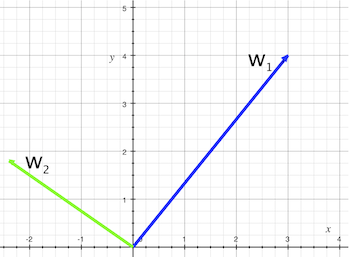
\includegraphics[scale=0.4]{Chap09VectorSpaceRnPart2/OrthognalVectors.png}  
\end{center}
Source: {\smaller \url{https://study.com/academy/lesson/the-gram-schmidt-process-for-orthonormalizing-vectors.html}}\\

Reading the values from the graph, we have 
$$ w_1=  \left[ \begin{array}{r}3 \\ 4  \end{array} \right],  w_2=  \left[ \begin{array}{r} -\frac{7}{3} \medskip \\   \frac{7}{4} \end{array} \right] \implies w_1 \bullet w_2 = w_1^\top w_2 = -3\frac{7}{3} + 4 \frac{7}{4} = 0 $$

It's very useful and amazing that this works for all vector spaces $\real^n$, as long as  $n\ge2$. Can you picture a right angle in $\real^{27}?$ Neither can your instructors, but later we'll see how useful the idea can be!
\end{tcolorbox}
\vspace*{.2cm}

\begin{tcolorbox}[title=\textbf{Pythagorean Theorem in $\boldsymbol{\real^n, n\ge2}$.}]
 Suppose that $w_1 \perp w_2$. Then,
$$||w_1 + w_2||^2 = ||w_1||^2 + ||w_2||^2. $$

\textbf{Remark} In the above plot, draw the line from $w_1$ to $w_2$ and call its length $c$; in addition, label the length of $w_1$ as $a$ and that of $w_2$ as $b$. Then yes, we have the classic relationship: $c^2 = a^2 + b^2$.
\end{tcolorbox}

\begin{example}
\label{ex:Pthagorean}
Why is this true? 
\end{example}

\textbf{Solution:} [\textbf{\RED Trigger Warning: This is a proof. You may want to skip it.]} Because $w_1 \perp w_2$, we know that $w_1 \bullet w_2=0,$ which means that $w_1^\top \cdot w_2 = w_2^\top \cdot w_1 = 0$. Finally, we recall that the norm-squared of a vector $v$ is  $||v||^2 = v^\top \cdot v$. Using these facts we grind out the computation and see
\begin{align*}
    ||w_1 + w_2||^2:&= (w_1+w_2)^\top \cdot (w_1+w_2)\\
    &= w_1^\top \cdot (w_1 + w_2) + w_2^\top \cdot (w_1 + w_2) \\
  &=w_1^\top \cdot w_1 +  w_1^\top \cdot w_2 +  w_2^\top \cdot w_1 +  w_2^\top \cdot w_2\\
    &= \underbrace{w_1^\top \cdot w_1}_{||w_1||^2} +  \underbrace{w_1^\top \cdot w_2}_{0} +  \underbrace{w_2^\top \cdot w_1}_{0} +  \underbrace{w_2^\top \cdot w_2}_{||w_2||^2} \\
    &= ||w_1||^2 + ||w_2||^2.
\end{align*}  \Qed

\begin{example}
\label{ex:perpendicular}
Determine which pairs of vectors, if any, are orthogonal
$$
u =  \left[ \begin{array}{r} 2 \\ 1 \\ -1\end{array} \right] , v= \left[ \begin{array}{r} 1\\ 3\\ 5 \end{array} \right], w= \left[ \begin{array}{r} -5 \\ 0 \\ 1\end{array} \right].$$
\end{example}
 \vspace*{.5cm}
 
\textbf{Solution} 
\begin{align*} 
u \bullet v & = u^\top \cdot v =\begin{bmatrix} 2 & 1 & -1\end{bmatrix} \cdot \begin{bmatrix} 1\\ 3\\ 5\end{bmatrix} = (2)(1) + (1) (3) + (-1)(5) = 0 \\
u \bullet w & = u^\top \cdot w =\begin{bmatrix} 2 & 1 & -1\end{bmatrix} \cdot \left[ \begin{array}{r} -5 \\ 0 \\ 1\end{array} \right] = (2)(-5) + (1) (0) + (-1)(1) = -11 \\
v \bullet w & = v^\top \cdot w =\begin{bmatrix} 1 & 3 & 5\end{bmatrix} \cdot \left[ \begin{array}{r} -5 \\ 0 \\ 1\end{array} \right] = (1)(-5) + (3) (0) + (5)(1) = 0,\\
\end{align*}
and hence, $u \perp v$, $u \not \perp w$, and $v \perp w$. In words, $u$ is orthogonal to $v$, $u$ is not orthogonal to $w$, and  $v$ is orthogonal to $w$. \Qed\\



%\subsection{Orthonormal Vectors}

\begin{tcolorbox}[sharp corners, colback=green!30, colframe=green!80!blue, title=\textbf{\Large Orthogonal and Orthonormal Vectors}]
A set of vectors $\{v_1, v_2, \ldots, v_n  \}$ is \textbf{orthogonal} if, for all $1 \le i, j \le n$, and $i\ne j$
\begin{equation}
    \label{eq:OrthognalVectors}
    v_i \bullet v_j =0.
\end{equation}
We can also write this as $v_i^\top v_j = 0$ or $v_i \perp v_j$.\\

A set of vectors $\{v_1, v_2, \ldots, v_n  \}$ is \textbf{orthonormal} if, 
\begin{itemize}
    \item they are orthogonal, and 
    \item for all $1 \le i \le n$, $||v_i||=1.$
\end{itemize}
\end{tcolorbox}

%\vspace*{.2cm}

\begin{example}
\label{ex:NormalizeLengthOne} 
Scale the vector $w$ so that its norm becomes one,
$$
w= \left[ \begin{array}{r} -5 \\ 0 \\ 1\end{array} \right].$$
\end{example}
 \vspace*{.5cm}
 
\textbf{Solution:} In general, if  $\alpha:= ||w|| \neq 0$ and we define $\tilde{w}:= \frac{1}{\alpha} w, $ then $$|| \tilde{w}||=1.$$
This is true because 
\begin{align*}
    || \tilde{w}||&= || \frac{1}{\alpha} \cdot {w}||\\
    &= \left|\frac{1}{\alpha}\right|\cdot || {w}|| ~~\text{(property of norms)}\\
    &= \frac{1}{\alpha} \cdot || {w}|| ~~(\frac{1}{\alpha}~\text{is positive})\\ 
    &= \frac{1}{\alpha} \cdot \alpha ~~(\text{definition of}~\alpha)\\
    &= \frac{\alpha}{\alpha} =1~~(\text{how scalar multiplication and division work})
\end{align*}
Hence, we need to form $\frac{w}{||w||}$, which gives
$$\tilde{w}:= \frac{1}{||w||} \cdot w = \frac{1}{\sqrt{26}}\left[ \begin{array}{r} -5 \\ 0 \\ 1\end{array} \right].$$ \Qed

\begin{example}
\label{ex:Orthonormal}
From Example~\ref{ex:perpendicular}, we already know that the set $\{u, v\}$ is orthogonal, that is, $u \perp v$. Make it an orthonormal set.
$$
u =  \left[ \begin{array}{r} 2 \\ 1 \\ -1\end{array} \right] , v= \left[ \begin{array}{r} 1\\ 3\\ 5 \end{array} \right].$$
\end{example}
 \vspace*{.5cm}
 
\textbf{Solution:} We need to normalize their lengths to one. We compute
\begin{align*}
    ||u||&= \sqrt{(2)^2 + (1)^2 + (-1)^2} = \sqrt{6}\\
    ||v||&= \sqrt{(1)^2 + (3)^2 + (5)^2} = \sqrt{35}
\end{align*}
and thus 
$$\left\{\tilde{u}:= \frac{1}{\sqrt{6}}  \left[ \begin{array}{r} 2 \\ 1 \\ -1\end{array} \right],  \tilde{v}:= \frac{1}{\sqrt{35}}  \left[ \begin{array}{r} 1\\ 3\\ 5 \end{array} \right] \right\}$$
is an orthonormal set of vectors. \Qed 

\vspace*{.2cm}

\begin{tcolorbox}[title=\textbf{\Large Orthonormal Vectors are Linearly Independent}]
For a set of vectors $\{ v_1, v_2, \ldots, v_k\}$ in $\real^n$, the following statements are true:
\begin{enumerate}
\renewcommand{\labelenumi}{(\alph{enumi})}
\setlength{\itemsep}{.2cm}
    \item  $\{ v_1, v_2, \ldots, v_k\}$ orthonormal implies it is linearly independent
    \item  $\{ v_1, v_2, \ldots, v_k\}$ orthogonal and  for all $i$, $v_i \neq 0_{n \times 1}$, together imply that the set is linearly independent
\end{enumerate}

\textbf{Remark:} In (b), the zero vector would be orthogonal to everything, but we needed to exclude it for us to have a linearly independent set. In (a), the lengths of the vectors being 1.0 excludes the zero vector. 
   
\end{tcolorbox}

\vspace*{.2cm}

What about the other direction? That is, given linearly independent vectors, can we construct a set of orthonormal vectors that span them? And if we can, would it even be useful? In Chapter~\ref{sec:gramSchmidt}, we address these questions.

\section{Orthogonal Matrices or Why Orthonormal Vectors are Super Useful}

This section is super cool! You will first learn about a kind of matrix whose inverse is equal to its transpose!! This is only the second inverse formula that your instructors want you to know and actually use!!!  \\

The hardest aspect of the this section is the vocabulary BECAUSE \textbf{a square matrix is orthogonal} if its columns are \textbf{orthonormal vectors}. I know, why not call them orthonormal matrices? Because that would be too easy? Because, by making it confusing, we can check who really knows what they are doing and who does not? No, it's another one of those historical accidents that we live with. Fortunately, the terminology \textit{orthonormal matrices} is used for a rectangular version of orthogonal matrices, and in applications, those are very important too.\\

Let's recall something about the sizes of matrices. If a matrix $Q$ is $n \times m$, then its transpose is $m \times n$. Therefore, we can form $Q^\top \cdot Q$ and have an $m \times m$ square matrix and we can form  $Q \cdot Q^\top$ and have an $n \times n$ square matrix.

\vspace*{0.2cm}
\begin{tcolorbox}[sharp corners, colback=green!30, colframe=green!80!blue, title=\textbf{\Large Orthonormal and Orthognal Matrices}]
An $n \times m$ rectangular matrix $Q$ is \textbf{orthonormal}: 
\begin{itemize}
    \item if $ n > m$ (tall matrix), its columns are orthonormal vectors, which is equivalent to $Q^\top \cdot Q = I_m;$ and
    \item if $ n < m$ (wide matrix), its rows are orthonormal vectors,  which is equivalent to $Q \cdot Q^\top = I_n.$
\end{itemize}
A square $n \times n$ matrix is \textbf{orthogonal} if $Q^\top \cdot Q = I_n$ and $Q \cdot Q^\top = I_n$, and hence, $Q^{-1} = Q^\top$.\\

\textbf{Remarks:} 
\begin{itemize}
    \item For a \textbf{square matrix}, $n =m$,  $(Q^\top \cdot Q = I_n) \iff (Q \cdot Q^\top = I_n) \iff (Q^{-1} = Q^\top). $
    \item For a tall matrix,  $n > m$, $(Q^\top \cdot Q = I_m) \notimplies (Q \cdot Q^\top = I_n).$
    \item For a wide matrix,  $m > n$, $ (Q \cdot Q^\top = I_n) \notimplies (Q^\top \cdot Q = I_m).$
\end{itemize}
\end{tcolorbox}

\begin{tcolorbox}[title=\textbf{\large Determinants of Orthogonal Matrices}]
Suppose that $Q$ is $n \times n$ and orthogonal so that $Q^\top Q = I_n$. Then 
$\left[\det(Q)\right]^2 = 1, $
and hence $\det(Q) = \pm 1.$ 
This follows from the determinant rule for a product of matrices, once you know for a square matrix $A$ that $\det(A^\top)=\det(A).$ 

$$Q~\text{ orthogonal} \implies \det(Q) = \pm 1.$$
\end{tcolorbox}



% \textbf{Remark:} The following are \textbf{equivalent} for a \textbf{square matrix} $Q$:
% \begin{itemize}
%     \item $Q$ is orthogonal;
%     \item $Q^\top \cdot Q = I_n$;
%      \item $Q \cdot Q^\top  = I_n$;
%      \item the columns of $Q$ are orthonormal; 
%      \item the rows of $Q$ are orthonormal; and
%      \item the columns of $Q^\top$ are orthonormal. 
% \end{itemize}


% If Q is not a square matrix, then the conditions QTQ = I and QQT = I are not equivalent. The condition QTQ = I says that the columns of Q are orthonormal. This can only happen if Q is an m × n matrix with n ≤ m (due to linear dependence). Similarly, QQT = I says that the rows of Q are orthonormal, which requires n ≥ m.

% There is no standard terminology for these matrices. They are sometimes called "orthonormal matrices", sometimes "orthogonal matrices", and sometimes simply "matrices with orthonormal rows/columns".



\section{Constructing Orthonormal Vectors: the Gram-Schmidt Process}

We already know how to normalize a set of orthogonal vectors to create a set of orthonormal vectors. Hence, we next look at how we might go about building a set of orthogonal vectors from vectors that are not orthogonal. We'll then learn the Gram-Schmidt Process, which is simply an algorithmic form of our process for building orthogonal vectors from non-orthogonal vectors. 

\subsection{Building Orthogonal Vectors}
\begin{example}
\label{ex:Orthogonalize} Suppose we have two vectors in $\real^3$,
$$u_1 = \left[\begin{array}{c}  1 \\ 1 \\1\end{array} \right]~\text{and}~u_2 = \left[\begin{array}{r}  1 \\ -1 \\2\end{array} \right].$$
It is easy to compute $u_1^\top \cdot u_2 = 2 \neq 0$, and thus the two vectors are not orthogonal. Find, if possible, two vectors $v_1$ and $v_2$ such that 
\begin{itemize}
    \item $v_1 \perp v_2$, 
    \item $\spanof{v_1} = \spanof{u_1}$, and
    \item $\spanof{v_1, v_2} = \spanof{u_1, u_2}$.
\end{itemize}  
In other words, $v_1$ and $v_2$ are orthogonal and yet they ``generate'' the same subspace as $u_1$ and $u_2$, which are not orthogonal. 
 \end{example}

\textbf{Solution:} If we set $v_1 = u_1$, then we trivially satisfy $\spanof{v_1} = \spanof{u_1}$. Let's see if we can write $v_2$ as a linear combination of $u_1$ and $u_2$ in such a way that $v_2 \bullet v_1 =0$ and $\spanof{v_1, v_2} = \spanof{u_1, u_2}$, where we have used the fact that 
$$v_1 \perp v_2 \iff v_1 \bullet v_2 = 0 \iff v_2 \bullet v_1 = 0. $$\\

\textbf{Step 1:} $v_1 := u_1 = \left[\begin{array}{c}  1 \\ 1 \\1\end{array} \right].$ \\

\textbf{Step 2:} $v_2 := u_2  - \alpha v_1$, where we seek to choose $\alpha$ such that $v_2 \bullet v_1 = 0$. We compute
\begin{align*}
    v_2 \bullet v_1 &  = \left( u_2  - \alpha v_1 \right) \bullet  v_1 \\
    &= u_2 \bullet v_1 - \alpha v_1 \bullet v_1.
\end{align*}
If $ v_1 \bullet v_1\neq 0$, then we can set $u_2 \bullet v_1 - \alpha v_1 \bullet v_1 = 0$ and solve for $\alpha$, namely
$$\alpha = \frac{u_2 \bullet v_1}{v_1 \bullet v_1}. $$
\\


\begin{tcolorbox}
\textbf{Important Formula to Build $\boldsymbol{v_1 \perp v_2}$ from $\boldsymbol{u_1}$ and $\boldsymbol{u_2}$ while Preserving Spans}
\begin{equation}
    \label{eq:OrthognalProjection01}
    \begin{aligned}
    v_1 &= u_1\\
    v_2 &= u_2 -  \left(\frac{u_2 \bullet v_1}{v_1 \bullet v_1}\right) v_1\\
    \\ 
    \spanof{v_1}&=\spanof{u_1}\\
    \spanof{v_1, v_2}&= \spanof{u_1, u_2}
     \end{aligned}
\end{equation}
\end{tcolorbox}

In our case, 
\begin{align*}
  u_2 \bullet v_1&= u_2^\top \cdot v_1 = \left[\begin{array}{ccc}  1 & -1 & 2 \end{array} \right] \cdot \left[\begin{array}{c}  1 \\ 1 \\1\end{array} \right] =  2 \bigskip \\
    v_1 \bullet v_1 &= u_1 \bullet u_1 = u_1^\top \cdot  u_1 = \left[\begin{array}{ccc}  1 & 1 & 1 \end{array} \right] \cdot \left[\begin{array}{c}  1 \\ 1 \\1\end{array} \right] = 3 \neq 0,
\end{align*}
and thus
$$\alpha = \frac{u_2 \bullet v_1}{v_1 \bullet v_1} = \frac{2}{3}. $$
and hence
$$v_2 = u_2  - \alpha v_1 = \left[\begin{array}{r}  1 \\ -1 \\2\end{array} \right] - \frac{2}{3} \left[\begin{array}{c}  1 \\ 1 \\1\end{array} \right] = \left[\begin{array}{r}  \frac{1}{3} \medskip \\ -\frac{5}{3} \medskip \\\frac{4}{3} \end{array} \right] $$

Did it work? Let's check if the vectors are orthogonal, that is, $v_1 \perp v_2,$
$$v_1 \bullet v_2 = v_1 ^\top \cdot v_2 =  \left[\begin{array}{ccc}  1 & 1  & 1\end{array} \right] \cdot \left[\begin{array}{r}  \frac{1}{3} \medskip \\ -\frac{5}{3} \medskip \\\frac{4}{3} \end{array} \right] = 0.$$

What about the span property? Well, as we noted when we started, $\spanof{v_1} = \spanof{u_1}$ because $v_1 = u_1$.\\

What about $\spanof{v_1,v_2}=\spanof{u_1,u_2}$? This part becomes a bit technical, so feel free to stop reading here and skip to the next subsection. We first ask, what does it even mean that $\spanof{v_1,v_2}=\spanof{u_1,u_2}$? Well, it means that if we take all linear combinations of the vectors $\{ v_1, v_2 \}$, we obtain the same ``set of vectors'' as taking  all linear combinations of the vectors $\{ u_1, u_2 \}$

We note that $v_1 = u_1$ and hence,
\begin{align}
    \label{eq:KeyToSpans01}
        v_2 &= u_2 -\alpha v_1 \\
    & \Updownarrow \nonumber \\
      \label{eq:KeyToSpans02}
    v_2 &= u_2 -\alpha u_1 \\
    & \Updownarrow \nonumber \\
      \label{eq:KeyToSpans03}
    u_2 &= v_2 +\alpha v_1 
\end{align}
From \eqref{eq:KeyToSpans02}, we have that 
$$\spanof{v_1, v_2} = \spanof{u_1,u_2 -\alpha u_1} \subset \spanof{u_1,u_2},$$
while from \eqref{eq:KeyToSpans03},
$$\spanof{u_1, u_2} = \spanof{v_1,v_2 +\alpha v_1} \subset \spanof{v_1,v_2}.$$
But for arbitrary subsets $S_1$ and $S_2$,
$$S_1 = S_2 \iff \left(S_1 \subset S_2~~\text{and}~~S_2 \subset S_1 \right) ,$$
and thus we have shown that $\spanof{v_1, v_2} = \spanof{u_1,u_2}$.\\

To be clear, this kind of proof was maybe a bit over the top for ROB 101! 
\Qed

% \subsection{Parallel-Orthogonal Decomposition of Vectors}

% Let $n\ge 2$, and let $u$ and $v$ be vectors in $\real^n$

% The process we followed to build a pair of orthogonal vectors has a very nice geometric interpretation. 

% $$v = v_{||} + v_{\perp} $$

% \begin{equation}
%     \label{eq:OrthognalDecomposition}
%     {\rm proj}_{u}(v):= \frac{u \bullet v}{u \bullet u} u
% \end{equation}

\subsection{Gram-Schmidt Process (aka the Gram-Schmidt Algorithm) for Building Orthonormal Vectors}
\label{sec:gramSchmidt}

Let's do one more step of producing orthogonal vectors. Let's assume that we have three linearly independent vectors $\{u_1, u_2, u_3\}$ and that we have already computed $v_1:=u_1$ and $v_2:= u_2 -  \left(\frac{u_2 \bullet v_1}{v_1 \bullet v_1}\right) v_1$ so that $v_1 \bullet v_2 = 0$. Let's now work on a third orthogonal vector. We define 
$$v_3:= u_3 - \alpha_1 v_2 - \alpha_2 v_2, $$
and try to find values for $\alpha_1$ and $\alpha_2$ so that $v_1\bullet v_3 = 0$ and $v_2 \bullet v_3 = 0$.

We compute 
\begin{align*}
    v_1\bullet v_3 & = v_1\bullet (u_3 - \alpha_1 v_1 - \alpha_2 v_2) \\
    & =  v_1\bullet u_3 - \alpha_1  v_1\bullet v_1 - \alpha_2  v_1\bullet v_2 \\
    & =  v_1\bullet u_3 - \alpha_1  v_1\bullet v_1 ~~(\text{because } v_1\bullet v_2 = 0)
\end{align*}
and 
\begin{align*}
    v_2\bullet v_3 & =  v_2\bullet (u_3 - \alpha_1 v_1 - \alpha_2 v_2) \\
    & =  v_2\bullet u_3 - \alpha_1  v_2\bullet v_1 - \alpha_2  v_2\bullet v_2 \\
    & =  v_2\bullet u_3 - \alpha_2  v_2\bullet v_2 ~~(\text{because } v_2\bullet v_1 = 0).
\end{align*}
Solving for $\alpha_1$ and $\alpha_2$ and substituting yields
\begin{equation}
    v_3:= u_3 - \frac{u_3 \bullet v_1}{v_1 \bullet v_1} v_1 - \frac{u_3 \bullet v_2}{v_2 \bullet v_2} v_2. 
\end{equation}

\begin{tcolorbox}[sharp corners, colback=green!30, colframe=green!80!blue, title=\textbf{\Large Gram-Schmidt Process}]
Suppose that that the set of vectors $\{ u_1, u_2, \ldots, u_m\}$ is linearly independent and you generate a new set of vectors by 
 \begin{equation}
 \label{eq:GramSchmidt}
 \begin{aligned}
 v_1 & = u_1 \\
 v_2 &= u_2 - \left(\frac{u_2 \bullet v_1}{v_1 \bullet v_1}\right) v_1 \bigskip \\
 v_3 &= u_3 -\left(\frac{u_3 \bullet v_1}{v_1 \bullet v_1}\right) v_1 - \left(\frac{u_3 \bullet v_2}{v_2 \bullet v_2}\right) v_2 \\
 & ~\vdots \\
	v_k &= u_k  - \sum_{i=1}^{k-1} \left(\frac{u_k \bullet v_i}{v_i \bullet v_i}\right) v_i~~~~~\text{(General Step)}
	\end{aligned}
\end{equation}

Then the set of vectors $\{ v_1, v_2,  \ldots, v_m\}$ is 
\begin{itemize}
    \item orthogonal, meaning, $i \neq j \implies v_i \bullet v_j = 0$
    \item span preserving, meaning that, for all $1 \le k \le m$, 
    \begin{equation}
        \label{eq:SpanPreserving}
        \spanof{v_1, v_2, \ldots, v_k} = \spanof{u_1, u_2, \ldots, u_k},
    \end{equation} 
    and
        \item linearly independent.
\end{itemize}

\textbf{Suggestion:} If you do not see the pattern in the steps of the Gram-Schmidt Algorithm, please compare \eqref{eq:GramSchmidt} to \eqref{eq:OrthognalProjection01}.
\end{tcolorbox}

\begin{tcolorbox}[title=\textbf{Preview of Basis Vectors}]
A set of vectors that is linearly independent and spans a given subspace is called a \textbf{basis for the subspace}. We are delaying the study of basis vectors until Chapter~\ref{chap:matrixFacts}. 
Equation~\eqref{eq:SpanPreserving} means that if you apply Gram-Schmidt to a set of \textbf{basis vectors}, then you will end with a \textbf{basis made of orthogonal vectors}. If you then normalize the \textbf{orthogonal basis}, you will produce an \textbf{orthonormal basis}!
\end{tcolorbox}





\begin{figure}[t!]
\centering
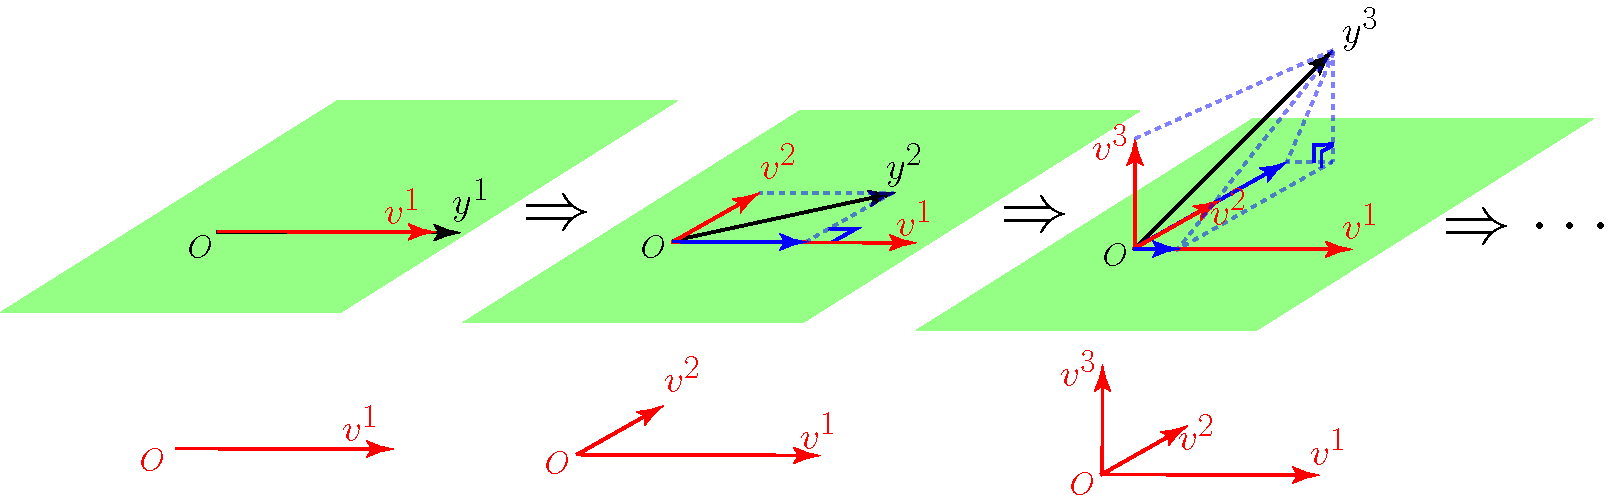
\includegraphics[width=0.9\textwidth]{Chap09VectorSpaceRnPart2/GramSchmidt.png}
\caption[]{Illustration of the Gram Schmidt Process. In the above, $y^i \leftrightarrow u_i$ and $v^i  \leftrightarrow v_i$. Image courtesy of Abhishek Venkataraman and Bruce Huang.} 
\end{figure}


\begin{example}
\label{ex:OrthonormalBasis}
You are given that the set below is a basis for $\real^3.$ Produce from it an orthonormal basis.
\begin{equation*}
	\{ u_1, u_2, u_3\} = \left\{
		\left[ \begin{array}{c} 1 \\ 1 \\ 0 \end{array} \right],
		\left[ \begin{array}{c} 1 \\ 2 \\ 3 \end{array} \right],
		\left[ \begin{array}{c} 0 \\ 1 \\ 1 \end{array} \right]
		\right\}
\end{equation*}

\end{example}

\textbf{Solution:} 

\textbf{Step 1} is to apply Gram-Schmidt to produce an orthogonal basis.
	\begin{align*}
		v_1 &= u_1 = \left[ \begin{array}{c} 1 \\ 1 \\ 0 \end{array} \right]\\
		v_1 \bullet v_1 &= (v_1)^\top v_1 = 2 ;\\
		\\
		v_2	&= u_2 - \frac{u_2 \bullet v_1}{v_1 \bullet v_1} v_1 \\
		&= \left[ \begin{array}{c} 1 \\ 2 \\ 3 \end{array} \right]
		- \underbrace{%
		   \left[ \begin{array}{ccc} 1 & 1 & 0 \end{array} \right]
		   \left[ \begin{array}{c} 1 \\ 2 \\ 3 \end{array} \right]%
		   }_{3}
		\frac{1}{2}
		   \left[ \begin{array}{c} 1 \\ 1 \\ 0 \end{array} \right]
		= \left[ \begin{array}{r}
			- \frac{1}{2} \medskip \\ \frac{1}{2} \medskip \\ 3
			\end{array} \right] \\
		v_2 \bullet v_2 &= v_2^\top v_2  = \frac{19}{2} \\
		\\
		v_3	&= u_3 - \frac{u_3 \bullet v_1}{v_1 \bullet v_1} v_1
			- \frac{u_3 \bullet v_2}{v_2 \bullet v_2} v_2 \\
		&= \left[ \begin{array}{c} 0 \\ 1 \\ 1 \end{array} \right]
		- \underbrace{%
		   \left[ \begin{array}{ccc} 1 & 1 & 0 \end{array} \right]
		   \left[ \begin{array}{c} 0 \\ 1 \\ 1 \end{array} \right]%
		   }_{1}
		\frac{1}{2}
		   \left[ \begin{array}{c} 1 \\ 1 \\ 0 \end{array} \right]
		- \underbrace{%
		   \left[ \begin{array}{ccc}
			-\frac{1}{2} & \frac{1}{2} & 3 \end{array} \right]
		   \left[ \begin{array}{c} 0 \\ 1 \\ 1 \end{array} \right]%
		   }_{3\frac{1}{2}}
		\frac{1}{\frac{19}{2}}
		   \left[ \begin{array}{r}
			-\frac{1}{2} \medskip \\ \frac{1}{2} \medskip \\ 3 \end{array} \right] \\
		&= \left[ \begin{array}{c} 0 \\ 1 \\ 1 \end{array} \right]
		- \left[ \begin{array}{c}
			\frac{1}{2} \\ \frac{1}{2} \\ 0 \end{array} \right]
		- \left[ \begin{array}{r}
			-\frac{7}{38} \medskip \\ \frac{7}{38} \medskip \\ \frac{21}{19}
			\end{array} \right]
		= \left[ \begin{array}{r}
			-\frac{6}{19} \medskip \\ \frac{6}{19} \medskip \\ -\frac{2}{19}
			\end{array} \right].
	\end{align*}
	
	Collecting the answers, we have
	\begin{equation*}
	\{ v_1, v_2, v_3\} = \left\{
		\left[ \begin{array}{c} 1 \\ 1 \\ 0 \end{array} \right],
		\left[ \begin{array}{r} -\frac{1}{2}  \medskip \\ \frac{1}{2} \medskip \\ 3 \end{array} \right],
	 \left[ \begin{array}{r}
			-\frac{6}{19} \medskip \\ \frac{6}{19} \medskip \\ -\frac{2}{19}
			\end{array} \right]
		\right\}
\end{equation*}

\textbf{Step 2:} Normalize to obtain an orthonormal basis (often useful to do this, but not always required).\\
	\begin{align*}
		\tilde{v}_1 &= \frac{v_1}{\| v_1 \|} = \frac{\sqrt{2}}{2} \left[ \begin{array}{c} 1  \\ 1  \\ 0 \end{array} \right]\\
		\tilde{v}_2 &= \frac{v_2}{\| v_2 \|} = \frac{\sqrt{38}}{38} \left[ \begin{array}{r} -1 \\ 1 \\ 6  \end{array} \right]\\
		\tilde{v}_3 &= \frac{v_3}{\| v_3 \|} = \frac{\sqrt{19}}{19} \left[ \begin{array}{r} -3  \\ 3\\ -1
			\end{array} \right]
	\end{align*}
	
	
\textbf{\BLUE All of this is quite tedious by hand, while being super fast and fun in Julia!}

\Qed

When we program the Gram-Schmidt process in Julia, we typically do the normalization as we go. When we normalize by ${v_i \leftarrow v_i/||v_i||}$, it follows that $v_i \bullet v_i =1$. Hence, the algorithm simplifies to the following.

\begin{tcolorbox}[title=\textcolor{red}{\Large \bf Gram-Schmidt Process with Normalization}]
Suppose that that the set of vectors $\{ u_1, u_2, \ldots, u_m\}$ is linearly independent and you generate a new set of vectors by applying Gram-Schmidt with normalization as we go, via 
 \begin{equation}
 \label{eq:GramSchmidtWithNormalization}
 \begin{aligned}
 v_1 & = u_1 \\
 v_1 & \leftarrow v_1/||v_1|| \\
 v_2 &= u_2 - \left(u_2 \bullet v_1 \right) v_1 \bigskip \\
 v_2 & \leftarrow  v_2 / ||v_2|| \\
 v_3 &= u_3 -\left( u_3 \bullet v_1 \right) v_1 - \left(u_3 \bullet v_2 \right) v_2 \\
 v_3 & \leftarrow  v_3/||v_3|| \\
 & ~\vdots \\
	v_k &= u_k  - \sum_{i=1}^{k-1} \left(u_k \bullet v_i\right) v_i~~~~~\text{(General Step)} \\
	v_k & \leftarrow  v_k/||v_k||,
	\end{aligned}
\end{equation}
where the symbol $\leftarrow $ means that we reassign the vector $v_k$ to its normalized value.\\

Then the set of vectors $\{ v_1, v_2,  \ldots, v_m\}$ is 
\begin{itemize}
    \item \textcolor{red}{\bf orthonormal}, meaning, $i \neq j \implies v_i \bullet v_j = 0$ \textcolor{red}{\bf and} for all $i$, $||v_i||=1$,
    \item span preserving, meaning that, for all $1 \le k \le m$, 
    $$
        \spanof{v_1, v_2, \ldots, v_k} = \spanof{u_1, u_2, \ldots, u_k},
    $$
    and
        \item linearly independent.
\end{itemize}
\end{tcolorbox}



\section{QR Factorization and Solutions of Linear Equations}
\label{sec:QRfactorization}

In Chapter~\ref{sec:SubspacesLines} we introduced the column span of an $n \times m$ matrix as the subspace of $\real^n$ generated by taking all of the linear combinations of the columns of the matrix. Applying Gram-Schmidt to the columns of a matrix yields the QR Factorization, which is one of the most advanced numerical methods for solving systems of linear equations.

\begin{tcolorbox}[sharp corners, colback=green!30, colframe=green!80!blue, title=\textbf{\Large QR Factorization}]
Suppose that $A$ is an $n \times m$ matrix with linearly independent columns. Then there exists an $n \times m$ matrix $Q$ with orthonormal columns and an upper triangular, $m \times m$, invertible matrix $R$ such that  $A=Q\cdot R$. Moreover, $Q$ and $R$ are constructed as follows:
\begin{itemize}
    \item Let $\{u_1, \ldots, u_m\}$ be the columns of $A$ with their order preserved so that 
    $$A=\left[ \begin{array}{cccc} u_1 & u_2 & \cdots& u_m \end{array} \right] $$
    \item $Q$ is constructed by applying the Gram-Schmidt Process to the columns of $A$ and normalizing their lengths to one,
    $$\{u_1, u_2, \ldots, u_m\} \xrightarrow[\text{Process}]{\text{Gram-Schmidt}} \{v_1, v_2, \ldots, v_m\}$$
 $$Q:=\left[ \begin{array}{cccc} \frac{v_1}{||v_1||} & \frac{v_2}{||v_2||} & \cdots& \frac{v_m}{||v_m||} \end{array} \right]  $$
 
 \item Because $Q^\top Q = I_m$, it follows that $A = Q \cdot R \iff R:=Q^\top \cdot A$. 
 
 \item Recalling that the columns of $A$ are linearly independent, if, and only if $x=0$ is the unique solution to $Ax=0$, we have that
 $$x=0 \iff Ax = 0 \iff Q \cdot R x = 0 \iff  Q^\top \cdot Q \cdot R x = Q^\top \cdot 0 \iff R x = 0 \iff \det(R) \neq 0,$$
 where the last step follows because $R$ is square.

\end{itemize}

\textbf{Remark:} Because $R$ is upper triangular, everything below its diagonal is zero. Hence, the calculation of $R$ can be sped up by extracting its coefficients from the Gram-Schmidt Process instead of doing the indicated matrix multiplication. We explore this in HW. 

\end{tcolorbox}

\vspace*{.2cm}

% The triangular structure of $R$ comes from the fact that for all $1 \le k \le m$,
% $$\spanof{u_1, u_2, \ldots, u_k}= \spanof{\frac{v_1}{||v_1||},  \frac{v_2}{||v_2||}, \ldots,  \frac{v_k}{||v_k||}},$$
% the ``nested structure'' that Gram-Schmidt naturally produces. From this nested structure, we have that
% \begin{align*}
%     u_1 &= r_{11} \frac{v_1}{||v_1||} \\
%     u_2 &= r_{12} \frac{v_1}{||v_1||} + r_{22} \frac{v_2}{||v_2||} \\
%     & \vdots \\
%     u_m&= r_{1m} \frac{v_1}{||v_1||} + r_{2m} \frac{v_2}{||v_2||} + \cdots +  r_{mm} \frac{v_m}{||v_m||},
% \end{align*}
% showing how the coefficients for $R$ can be obtained from the Gram-Schmidt process itself, instead of through the matrix multiplication $R=Q^\top \cdot A$. 

\begin{example}
\label{ex:QRFactorization} Compute the QR Factorization of $A=	\left[ \begin{array}{ccc} 1 & 1 & 0 \
\\ 1 & 2 & 1\\
0 & 3 & 1\end{array} \right].$
\end{example}

\textbf{Solution:} We extract the columns of $A$ and obtain
\begin{equation*}
	\{ u_1, u_2, u_3\} = \left\{
		\left[ \begin{array}{c} 1 \\ 1 \\ 0 \end{array} \right],
		\left[ \begin{array}{c} 1 \\ 2 \\ 3 \end{array} \right],
		\left[ \begin{array}{c} 0 \\ 1 \\ 1 \end{array} \right]
		\right\}
\end{equation*}
From Example~\ref{ex:OrthonormalBasis}, we have that\
$$
\left\{ 
		\tilde{v}_1 = \frac{v_1}{\| v_1 \|} = \frac{\sqrt{2}}{2} \left[ \begin{array}{c} 1  \\ 1  \\ 0 \end{array} \right], 
		\tilde{v}_2 = \frac{v_2}{\| v_2 \|} = \frac{\sqrt{38}}{38} \left[ \begin{array}{r} -1 \\ 1 \\ 6  \end{array} \right], 
		\tilde{v}_3 = \frac{v_3}{\| v_3 \|} = \frac{\sqrt{19}}{19} \left[ \begin{array}{r} -3  \\ 3\\ -1 \end{array} \right]
\right\}
$$	
and therefore,
$$Q\approx \left[ \begin{array}{rrr} 
 0.707107 &  -0.162221  & -0.688247 \\
 0.707107  &  0.162221  & 0.688247\\
 0.000000  &       0.973329   & -0.229416
  \end{array} \right]$$
  and
$$R = Q^\top \cdot A \approx   \left[ \begin{array}{ccc} 
1.41421  &    2.12132    & 0.707107 \\
0.00000 & 3.08221    &   1.13555 \\
0.00000 &  0.00000 & 0.458831
  \end{array} \right].$$\\

  As a numerical check, we also compute how close $Q^\top$ is to being a matrix inverse of $Q$,
  $$Q^\top \cdot Q- I=  \left[ \begin{array}{rrr}
 -2.22045e-16 &  9.71445e-17  & 1.11022e-16\\
  9.71445e-17  & 0.00000  e-17    &    -2.49800e-16\\
  1.11022e-16 & -2.49800e-16  &    0.00000  e-17
 \end{array} \right].$$
 In addition, we check that $\det(Q)=-1.0$.
\Qed \\

 
 
\vspace*{.2cm}

\begin{tcolorbox}[sharp corners, colback=green!30, colframe=green!80!blue, title=\textbf{\Large Suggested Pipeline: Solutions of Linear Equations via the QR Factorization}]
Suppose that $A$ is $n \times n$ and its columns are linearly independent. Let $A=Q \cdot R$ be its QR Factorization. Then
\begin{equation}
    \label{eq:SolvingLSviaQR}
    (Ax = b) \iff (Q \cdot Rx = b) \iff (R x = Q^\top b).
\end{equation}
Hence, whenever $\det(A) \neq 0$, the suggested ``pipeline'' for solving $Ax=b$ is
\begin{itemize}
    \item factor $A =: Q \cdot R$,
    \item compute $\overline{b}:= Q^\top b$, and then 
    \item solve $R x = \overline{b}$ via back substitution.  
\end{itemize}
\end{tcolorbox}

\begin{example}
\label{ex:QRSolveAxequalsb} Use the suggested pipeline to solve the system of linear equations
$$\underbrace{\left[ \begin{array}{ccc} 1 & 1 & 0 \
\\ 1 & 2 & 1\\
0 & 3 & 1\end{array} \right]}_{A} x =  
\underbrace{\left[ \begin{array}{c}
1 \\  4 \\  7\end{array} \right]}_{b}.$$

\end{example}

\textbf{Solution:} From Example~\ref{ex:QRFactorization}, 
$$ \underbrace{\left[ \begin{array}{ccc} 1 & 1 & 0 \
\\ 1 & 2 & 1\\
0 & 3 & 1\end{array} \right]}_{A} = \underbrace{\left[ \begin{array}{rrr} 
 0.707107 &  -0.162221  & -0.688247 \\
 0.707107  &  0.162221  & 0.688247\\
 0.000000  &       0.973329   & -0.229416
  \end{array} \right]}_{Q} \cdot 
\underbrace{\left[ \begin{array}{ccc} 
1.41421  &    2.12132    & 0.707107 \\
0.00000 & 3.08221    &   1.13555 \\
0.00000 &  0.00000 & 0.458831
  \end{array} \right]}_{R}. $$
  
We form
$$\overline{b}:= Q^\top b =  \left[ \begin{array}{r}
 3.53553\\
 7.29996\\
 0.45883
  \end{array} \right]
$$
and then use back substitution to solve
$$ \underbrace{\left[ \begin{array}{ccc} 
1.41421  &    2.12132    & 0.707107 \\
0.00000 & 3.08221    &   1.13555 \\
0.00000 &  0.00000 & 0.458831
  \end{array} \right]}_{R} x =  \underbrace{\left[ \begin{array}{r}
 3.535534\\
 7.299964\\
 0.458831
  \end{array} \right]}_{\overline{b}},$$
  which yields
  $$ x = \left[ \begin{array}{r}
 -1\\
 2\\
 1
  \end{array} \right]. $$

\Qed\\


\begin{tcolorbox}[sharp corners, colback=green!30, colframe=green!80!blue, title=\textbf{\Large Least Squares via the QR Factorization}]
Suppose that $A$ is $n \times m$ and its columns are linearly independent (tall matrix). Let $A=Q \cdot R$ be its QR Factorization. Then $A^\top A = R^\top \cdot Q^\top \cdot Q \cdot R = R^\top\cdot R$ and thus 
\begin{equation}
    \label{eq:SolvingAxbSquareQR}
    (A^\top \cdot Ax = A^\top b) \iff (R^\top \cdot R x = R^\top \cdot Q^\top b) \iff (R x = Q^\top b),
\end{equation}
where we have used the fact that $R$ is invertible. 
Hence, whenever the columns of $A$ are linearly independent, the suggested ``pipeline'' for  computing a least squared error solution to $Ax=b$ is 
\begin{itemize}
    \item factor $A =: Q \cdot R$,
    \item compute $\overline{b}:= Q^\top b$, and then 
    \item solve $R x = \overline{b}$ via back substitution.  
\end{itemize}
\end{tcolorbox}

Yes! The two pipelines are identical!! Your surprise will be tempered when you go back to our discussion of least squared error solutions of linear equations where we noted that if $A$ is square and its determinant is non-zero, then
$$(Ax=b) \iff (A^\top \cdot A x = A^\top b). $$
The only difference in the two cases is that when $A$ is square, $Q$ is an orthogonal matrix whereas, when $A$ is a tall matrix, then $Q$ is an orthonormal matrix. Yes, it's a subtle difference! Is it an important difference? Not really, as long as you only form $Q^\top \cdot Q$ and you avoid $Q \cdot Q^\top.$

\begin{example}
\label{ex:LeastSqaresQR}
We rework Example~\ref{ex:LeastSqauredLinearEquations} from 
Chapter~\ref{sec:LeastSqauresGeneral}, where we seek a least squared error solution to the system of linear equations
\begin{equation}
\label{eq:LeastSquareSolExampleAgain}
\underbrace{\left[\begin{array}{rrr}
 1.0 & 1.0 \\
 2.0 & 1.0 \\
 4.0 & 1.0 \\
 5.0 & 1.0 \\
 7.0  & 1.0
 \end{array}\right]}_{A} \underbrace{\left[\begin{array}{c}
x_1 \\ x_2  \end{array}\right]}_{x} =  \underbrace{\left[\begin{array}{r}
4 \\  8 \\ 10 \\ 12 \\ 18 \end{array}\right]}_{b}.
\end{equation}

\end{example}

\textbf{Solution:} Since the columns of $A$ are linearly independent, we compute the QR factorization of $A$ and obtain
$$ Q= \left[\begin{array}{lr}
0.102598  &  0.730297 \\
 0.205196 &   0.547723 \\
 0.410391  &  0.182574 \\
 0.512989  & 0.000000 \\
 0.718185  & -0.365148 \\
 \end{array}\right], R =  \left[\begin{array}{lr}
    9.74679  &      1.94936\\
 0.0  &  1.09545
 \end{array}\right], ~\text{and}~ Q^\top\cdot b =   \left[\begin{array}{l} 25.23906 \\ 2.556038\end{array}\right].
 $$ 
 We then use back substitution to solve
 $$\left[\begin{array}{lr}
    9.74679  &      1.94936\\
 0.0  &  1.09545
 \end{array}\right] x = \left[\begin{array}{l} 25.23906 \\ 2.556038\end{array}\right]$$
which yields
$$x^*= \left[\begin{array}{l}2.1228\\2.3333\end{array}\right]. $$ 
\Qed

For small made-up problems like this one, there is no real numerical advantage to using a sophisticated solution like our ``suggested pipeline''. In real engineering, it makes a huge difference. Prof. Grizzle's and Ghaffari's students use the suggested pipeline, either as given with QR or its equivalent via LU, when working with Cassie Blue.\\

\begin{tcolorbox}[sharp corners, colback=green!30, colframe=green!80!blue, title = \textbf{\Large LU vs QR: Which is Better?} ]
The answer seems to be highly situational. One of the giants of Linear Algebra education, Prof. Gilbert Strang, writes ``The LU vs QR choice comes up for example with least squares equations  $A^\top \cdot A x = A^\top b$.  If we actually form $A^\top \cdot A$ and solve by LU, it is a bit faster than using $A = QR$, but less [numerically] stable :  We could do $R^\top \cdot Q^\top \cdot  Q \cdot R x = R^\top \cdot Q^T b$, which is just $R x = Q^\top b$ and [is] more stable. Cleve Moler [a co-founder of the Mathworks] and I are testing various methods for underdetermined systems with $n >> m$
(because deep learning often has more parameters than equations to determine them, and it still works).''
\end{tcolorbox}


\section{Underdetermined Equations or What to do When Ax=b has an Infinite Number of Solutions?}
\label{sec:MinNormSolution2LinearEquations}

We consider $Ax=b$ and recall what we know about its solutions:
\begin{itemize}
    \item $b \in \colspanof{A} \iff$ a solution exists;
    \item the solution is unique if, and only if, the columns of $A$ are linearly independent; and thus
    \item if there exists one solution and the columns of $A$ are linearly dependent, then there exist an infinite number of solutions.
\end{itemize} 

\begin{tcolorbox}[title=\textbf{\Large Underdetermined Equations}]
The columns of $A$ will be linearly dependent when $Ax=b$ has fewer equations than unknowns. In other words, $A$ is $n \times m$ and $m > n$; we've been calling these wide matrices: more columns than rows. When dealing with an equation $Ax=b$ with fewer equations than unknowns, one says that it is \textbf{underdetermined}. Why? Because, to determine $x$ uniquely, at a minimum, we need as many equations as unknowns.\\

\textbf{Is there a difference between being underdetermined and having an infinite number of solutions?} Yes. It's possible to be underdetermined and have no solution at all when $b \not \in \colspanof{A}$. If the rows of $A$ are linearly independent, then 
$$Ax=b ~~\text{is underdetermined}~~\iff ~Ax=b~~\text{has an infinite number of solutions.}$$
The rows of $A$ being linearly independent is equivalent to the columns of $A^\top$ being linearly independent.
\end{tcolorbox}
\vspace*{.2cm}
When $Ax=b$ has an infinite number of solutions, is there a way that we can make one of them appear to be more interesting, more special, or just flat out ``better'' than all the other solutions? Is there a property that we could associate with each solution and optimize our choice of solution with respect to that property? The most common approach is to choose the solution with minimum norm! \\

\begin{tcolorbox}[sharp corners, colback=green!30, colframe=green!80!blue, title=\textbf{\Large Minimum Norm Solution to Underdetermined Equations}]
Consider an underdetermined system of linear equations $Ax=b$. If the rows of $A$ are linearly independent (equivalently, the columns of $A^\top$ are linearly independent), then 
\begin{equation}
\label{eq:MinNormUnderDetermined}
    x^\ast = \argmin_{Ax=b} ||x|| \iff x^\ast = A^\top\cdot (A \cdot A^\top)^{-1} b 
    \iff x^\ast = A^\top \alpha~~\text{and}~~A\cdot A^\top \alpha =b.
\end{equation}
We recommend that the minimum norm solution $x^\ast$ be computed with the right-hand side of \eqref{eq:MinNormUnderDetermined} so that the matrix inverse is avoided, but for small problems, the middle answer is fine. \\

Suppose we do the QR Factorization of $A^\top$ instead of $A$ itself, so that
$$ A^\top = Q \cdot R.$$
Because the columns of $A^\top$ are linearly independent, $R$ is square and invertible. It follows that $A = R^\top \cdot Q^\top$ and $A \cdot A^\top = R^\top \cdot R$ because $Q^\top \cdot Q = I$. Using these facts, \eqref{eq:MinNormUnderDetermined} can be rewritten as
\begin{equation}
\label{eq:MinNormUnderDeterminedQR}
    x^\ast = \argmin_{Ax=b} ||x|| \iff x^\ast = Q \cdot \left( R^\top \right)^{-1} b 
    \iff x^\ast = Q \beta~~\text{and}~~R^\top \beta =b.
\end{equation}
We note that $R^\top$ is lower triangular, and thus $R^\top \beta = b$ can be solved via forward substitution. Hence, our suggested ``pipeline'' for underdetermined problems $Ax=b$ is
\begin{itemize}
    \item Check that the columns of $A^\top$ are linearly independent and compute $A^\top = Q \cdot R.$
    \item Solve $R^\top \beta = b$ by forward substitution.
    \item $x^\ast = Q \beta.$
\end{itemize}

\textbf{Remark:} In case you are curious, $\beta$ in \eqref{eq:MinNormUnderDeterminedQR} is related to $\alpha$ in \eqref{eq:MinNormUnderDetermined} by $\beta = R \alpha. $ The two $x^\ast$ are the same!\\

\end{tcolorbox}

\begin{example}
\label{ex:QRSolveUnderdetermined} Use the suggested pipeline to determine a minimum norm solution to the system of underdetermined equations
$$\underbrace{\left[ \begin{array}{ccc} 1 & 1 & 0 \
\\ 1 & 2 & 1\\
\end{array} \right]}_{A} x =  
\underbrace{\left[ \begin{array}{c}
1 \\  4 \end{array} \right]}_{b}.$$
\end{example}

\textbf{Solution:} The columns of $A^\top$ are linearly independent and we compute the QR Factorization to be
$$A^\top = \left[ \begin{array}{cc} 1 & 1\\ 
1 & 2\\
0 & 1
\end{array} \right] =  \underbrace{\left[ \begin{array}{rr}
 0.707107 & -0.408248 \\
 0.707107  & 0.408248  \\
 0.000000      &  0.816497
 \end{array} \right]}_{Q} \cdot
  \underbrace{\left[ \begin{array}{rr}
 1.41421  &    2.12132 \\
 0.00000 & 1.22474
 \end{array} \right]}_{R}.
$$
We solve $R^\top \beta = b$ and obtain 
$$ \beta = \left[ \begin{array}{r}
 0.70711 \\
 2.04124
  \end{array} \right],$$
  and then $x^\ast = Q \beta$ to arrive at the final answer
  $$x^\ast = \left[ \begin{array}{r}
 -0.33333 \\
  1.33333  \\
  1.66667 \\ 
  \end{array} \right]. $$
  To verify that $x^\ast$ is indeed a solution, we substitute it into  $Ax-b $ and obtain
  $$Ax^\ast -b =  \left[ \begin{array}{r}
     0.000000~~\\
 -4.441 e\mbox{-}16
  \end{array} \right],$$
which looks like a pretty good solution! 
\Qed

\vspace*{.2cm}

\begin{tcolorbox}[title = \textbf{A Quick Check}]
Is $x^\ast$ in Example~\ref{ex:QRSolveUnderdetermined} the solution of smallest norm? Of course! Don't you trust us? To which you respond, ``of course not!'' \\

Let's see about that. What are other solutions? We claim they all have the form
$x^\ast + \bar{x}$, where $A \bar{x} = 0$, because then 
$$A(x^\ast + \bar{x}) = A x^\ast + A \bar{x} = b + 0 = b.$$
Indeed, we compute that all solutions to $Ax = 0$ have the form
$$ \bar{x} = \gamma \left[ \begin{array}{r}
1 \\
-1 \\ 
 1  \end{array} \right],$$
 and therefore, all solutions to $Ax=b$ have the form
 $$x_{\rm sol} = x^\ast + \bar{x}. $$
 The next thing we can check is that for all $\gamma \in \real,$ $x^\ast \perp \bar{x}$, and hence, by the Pythagorean Theorem, we have that
 $$||x_{\rm sol}||^2 = ||x^\ast + \bar{x}||^2 =  ||x^\ast||^2 + ||\bar{x}||^2 = ||x^\ast||^2 + {3} \gamma^2.$$
 It follows that $$\min_{\gamma} || x_{\rm sol}||^2 = \min_{\gamma} \left( ||x^\ast||^2 + {3} \gamma^2  \right) =  ||x^\ast||^2 + \min_{\gamma} \left({3} \gamma^2\right)$$
and thus the minimum occurs for $\gamma = 0$. Hence, $x^\ast$ is indeed the minimum norm solution! 
\end{tcolorbox}

\vspace*{.2cm} 

\textbf{Optional Read:} The Pythagorean Theorem is a powerful ally when one seeks to establish minimum norm properties. We use it to show that \eqref{eq:MinNormUnderDetermined} has the claimed minimum norm property among all solutions of $Ax=b$. All of the ideas are actually present in our analysis of Example~\ref{ex:QRSolveUnderdetermined}. Here we sketch the general case.\\

The proposed minimum norm solution to $Ax=b$ has the form $x^\ast = A^\top \alpha$, which is a linear combination of the columns of $A^\top$. Indeed, for $A$ an $n \times m$ matrix we write
$$A = \left[ \begin{array}{c}
a^{\rm row}_1 \\
\vdots\\
a^{\rm row}_n
  \end{array} \right]~~\text{and}~~\alpha=\left[ \begin{array}{c}
\alpha_1 \\
\vdots \\
\alpha_n
  \end{array} \right]~~\text{so that}~~A^\top \alpha = 
    \left[ \begin{array}{ccc}
\left(a^{\rm row}_1\right)^\top &
\cdots & 
\left(a^{\rm row}_n\right)^\top
  \end{array} \right]
  \left[ \begin{array}{c}
\alpha_1 \\
\vdots \\
\alpha_n
  \end{array} \right]=
  \alpha_1 \left(a^{\rm row}_1\right)^\top + \cdots +  \alpha_n \left(a^{\rm row}_n \right)^\top.$$
  We next note that $A \bar{x} = 0$ if, and only if, for all $1 \le i \le n$,
  $a^{\rm row}_i \bar{x} = 0$, which is equivalent to $ ( a^{\rm row}_i )^\top \perp \bar{x}.$ Hence, we have that
  $$x^\ast \perp \bar{x} $$
  A general solution to $Ax=b$ can be written as $x_{\rm sol}= x^\ast + \bar{x}$, where $\bar{x}$ is any solution to $Ax=0$. Applying the Pythagorean Theorem we have $$||x_{\rm sol}||^2 = || x^\ast + \bar{x}||^2 = || x^\ast||^2 + || \bar{x}||^2.$$
Because $|| x^\ast||^2 + || \bar{x}||^2$ is smallest for $\bar{x}=0$, it follows that
  $$ \min_{ \bar{x} } ||x_{\rm sol}||^2 =  \min_{ \bar{x} }  || x^\ast||^2 + || \bar{x}||^2 =  || x^\ast||^2, $$
  which shows that \eqref{eq:MinNormUnderDetermined} really is the minimum norm solution.

  
  
\section{Steering a Mobile Robot as a Practical Example of an Underdetermined System of Linear Equations} 
\label{sec:PracticalUnderDeterminedExample}

We first develop a model of a mobile robot. We assume that the robot moves in $\real^2$ with its $x$-position denoted $p^x$ and $y$-position denoted $p^y$. We gather these two coordinates together and write them as a vector
\begin{equation}
   p:= \begin{bmatrix} p^x \\ p^y \end{bmatrix},
\end{equation}
which is typically called the \textbf{state of the robot}. 
Because we are modeling a mobile robot, its position/state changes with time. For reasons explained in Appendix~\ref{chap:ODE} of our textbook, we discretize time into uniform samples. So, we let $\delta t >0$ be some base unit or duration of time, typically small, and define $t_0, t_1, t_2, \ldots, t_k, \ldots$, where $t_k:=k \delta t$. We denote the robot's position at time $t_k$ by
\begin{equation}
\label{eq:stateVariablesMobileRobot}
   p_k:= \begin{bmatrix} p^x_k \\ p^y_k \end{bmatrix};
\end{equation}
in other words, the subscript $k$ keeps track of time. With this notation, $p_0$ will be the initial position of the robot in the plane (i.e., in $\real^2$) at time $t_0$. \\

\begin{figure}[htb]%
\centering
\subfloat[]{%
    \label{fig:MobileRobotsA}%
\centering
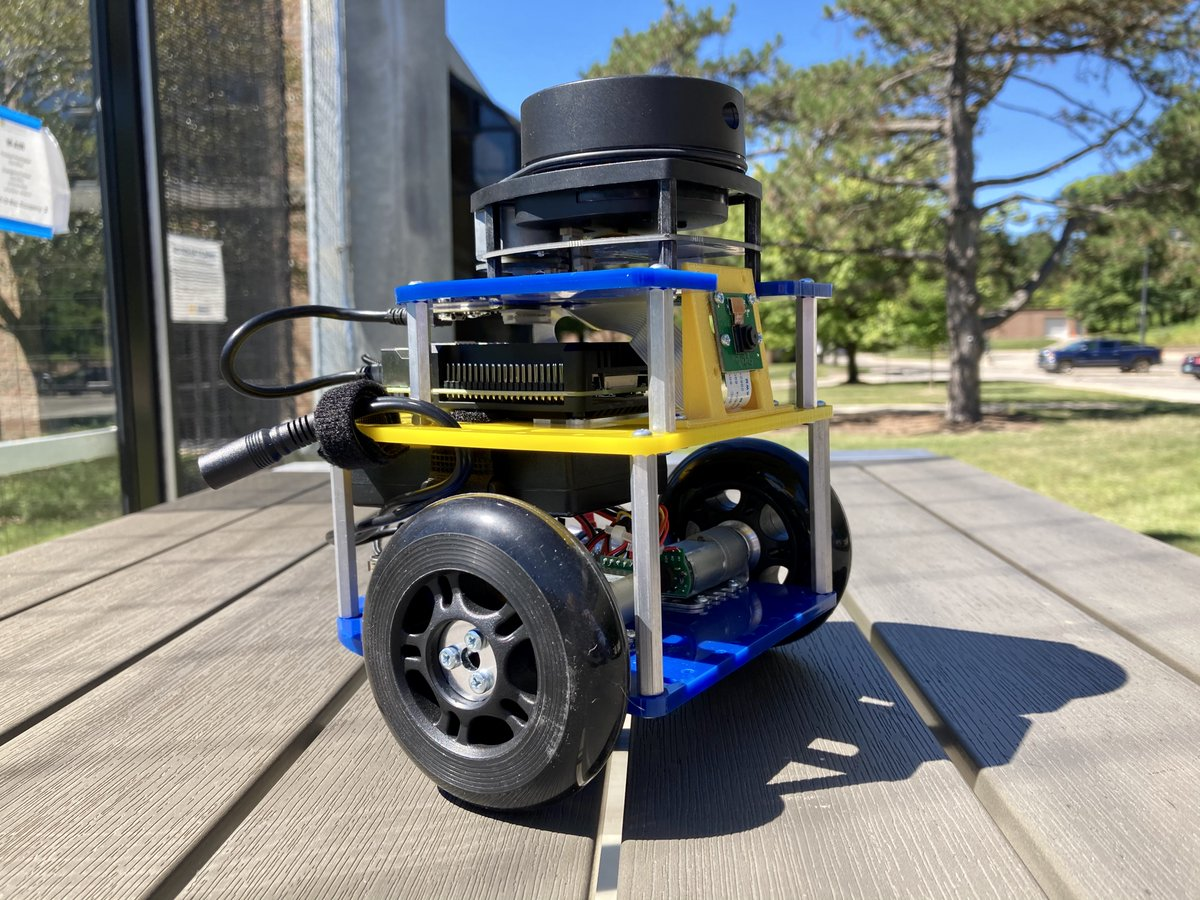
\includegraphics[width=0.4\textwidth]{Chap09VectorSpaceRnPart2/Mbot.jpg}
}
\hspace{5pt}%
\subfloat[]{%
    \label{fig:MobileRobotsB}%
	\centering
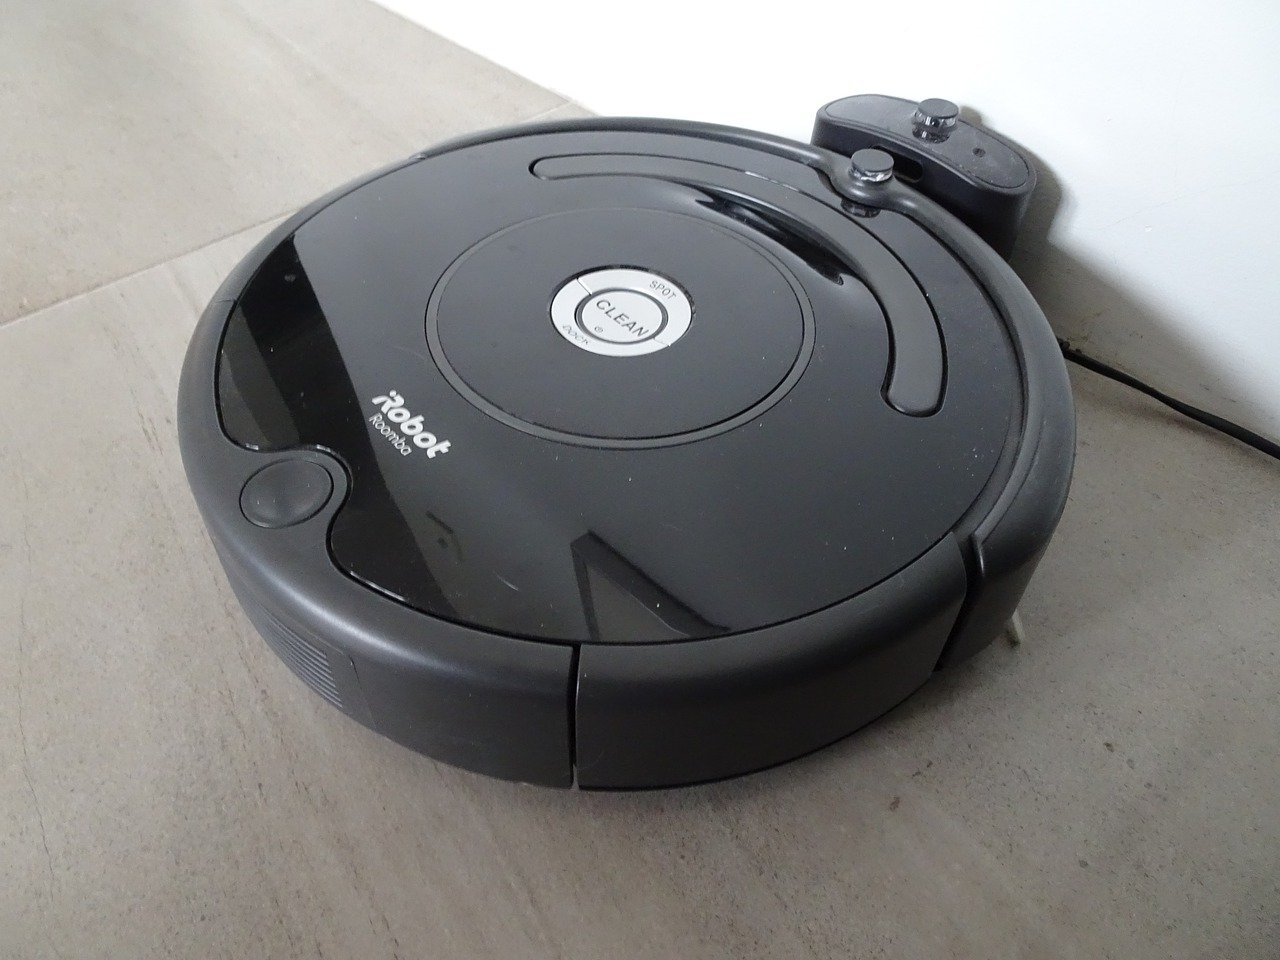
\includegraphics[width=0.40\textwidth]{Chap09VectorSpaceRnPart2/ROOMBArobot-vacuum-cleaner-5311418_1280.jpg}}%
\caption[]{Two mobile robots. (a) Michigan M-bot as used in ROB 103, ROB 320, ROB 330, and ROB 550. (b) iRobot's roomba vacuum cleaning robot.}
    \label{fig:MobileRobots}
\end{figure}


The next thing we posit is that our mobile robot has ``dynamics'', meaning that its state at time $t_{k+1}$ can be expressed as a function of its state at time $t_k$ and any motor commands that we provide. Because we are studying linear algebra, we assume that 
\begin{equation}
\label{eq:DynamicModelMobileRobot}
    p_{k+1} = A p_k + B u_k,
\end{equation}
where $u_k\in \real^2$ is a pair of motor commands, the $2 \times 2$ matrix $B$ distributes the motor commands to effect motion of the robot (that is, change its next position), and $A$ is a $2 \times 2$ matrix that in a realistic model would capture the mass of the robot, the inertia of rotating parts, and other effects from physics. \\


Even though the following values are not so realistic, we'll go ahead and assume that
\begin{equation}
    \begin{aligned}
    \delta t &= 0.1 \\
    A &= I_{2 \times 2} + \delta t \left[ \begin{array}{rr} 0.0 & -0.5 \\ 0.5 & 0.0 \end{array}  \right] \\
    B&= \delta t I_{2 \times 2},
    \end{aligned}
\end{equation}
so that the we can focus on the process of steering the robot and not the complexity of the robot's model. \\

\begin{figure}[h]%
\centering
\subfloat[]{%
    \label{fig:MobileRobotTrajectoriesA}%
\centering
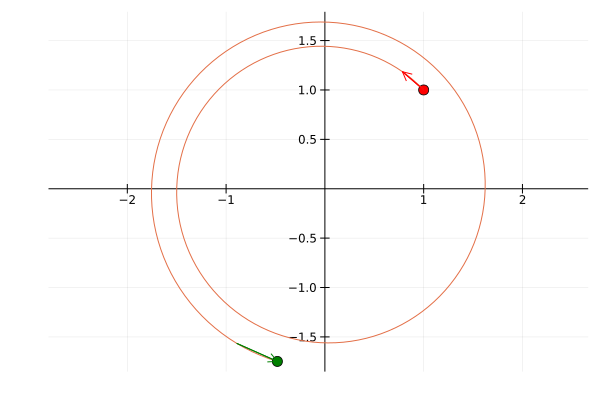
\includegraphics[width=0.5\textwidth]{Chap09VectorSpaceRnPart2/WonderingMobileRobot.png}
}
\hspace{5pt}%
\subfloat[]{%
    \label{fig:MobileRobotTrajectoriesB}%
	\centering
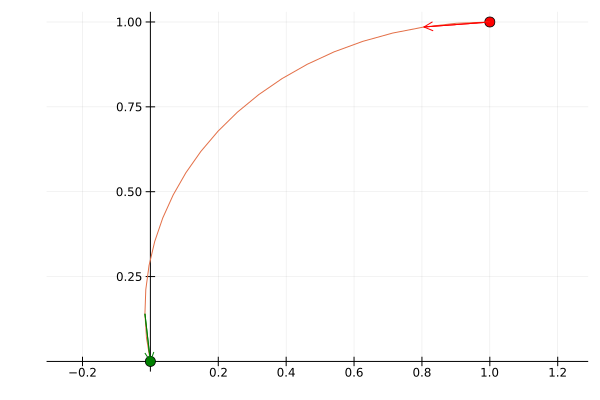
\includegraphics[width=0.40\columnwidth]{Chap09VectorSpaceRnPart2/ControlledMobileRobot.png}}%
\caption[]{Controlling the motion of a mobile robot. (a) shows the evolution of the robot if we apply motor commands that are identically zero. With our chosen model, the robot wanders around like a Roomba.  (b) shows us deliberately steering the robot to the origin using methods from Linear Algebra. The problem turns out to be one of an underdetermined system of linear equations. }
    \label{fig:MobileRobotTrajectories}
\end{figure}

\newpage

\textbf{Why do we want a model? So that we can predict the future behavior of the robot.} Not only do we have a way to compute the state at the next time instant based on the current state and current input, we can also iterate forward and \textbf{predict} the state at some future time, say $N$, as a function of a hypothesized input sequence, $\{u_0, u_1, \ldots, u_{N-1} \}$ as follows
\begin{equation}
    \label{eq:MobileRobotFutureStates}
\begin{aligned}
    p_0 &= \text{ given initial position} \nonumber\\
    p_1 &= A p_0 + B u_0 \nonumber\\
    p_2 &= A p_1 + B u_1 = A(A p_0 + B u_0 ) + B u_1 = A^2 p_0 + A B u_0 + B u_1 \nonumber\\
    p_3 &= A p_2 + B u_2 = A(A^2 p_0 + A B u_0 + B u_1) + B u_2 = A^3 p_0 + A^2 B u_0 + A B u_1 + B u_2 \nonumber\\
    &\vdots \nonumber\\
    p_N &= A^N p_0 + A^{N-1} B u_0 + A^{N-2} B u_1 + \cdots + A B u_{N-2} + B u_{N-1}
\end{aligned}
\end{equation}

That's a lot of symbols, but what do they tell us? Suppose we start the robot at 
$$ p_0:= \begin{bmatrix} p^x_0 \\ p^y_0 \end{bmatrix} = \begin{bmatrix} 1.0\\ 1.0 \end{bmatrix}$$
and we set the motor commands to be identically zero. Then we can predict how the robot will move ``on its own''. Figure~\ref{fig:MobileRobotTrajectories}-(a) shows the evolution of our robot for $0 \le t_k \le 20$ seconds, that is, $0 \le k \le 200$ (because $\delta t=0.1$). When we are not actively modifying its trajectory, our robot is a bit like a wandering Roomba, spiraling outward trying to get its bearings! \\

Let's suppose we want to actively steer the robot to the origin in $2$ seconds, that is, 
$$ p_N:= \begin{bmatrix} p^x_N \\ p^y_N \end{bmatrix} = \begin{bmatrix} 0.0\\ 0.0 \end{bmatrix},$$
where $N=20$. Then we are seeking a solution to the equation
\begin{equation}
\label{eq:FinalConditionUnderDetermined}
\begin{aligned}
    p_N &= A^N p_0 + A^{N-1} B u_0 + A^{N-2} B u_1 + \cdots + A B u_{N-2} + B u_{N-1}\\
    & \Updownarrow\\
     p_N - A^N p_0  & = A^{N-1} B u_0 + A^{N-2} B u_1 + \cdots + A B u_{N-2} + B u_{N-1} \\
      & \Updownarrow\\
       p_N - A^N p_0 &= \left[\begin{array}{ccccc}  A^{N-1} B  & A^{N-2} B  &\cdots & A B  & B  \end{array}  \right] \left[\begin{array}{c}   u_0 \\ u_1 \\ \vdots \\  u_{N-2} \\ u_{N-1} \end{array}  \right],
\end{aligned}
\end{equation} 
where the unknowns are the control decisions $u_{\rm seq}:=(u_0, u_1, \ldots, u_{N-2}, u_{N-1})$. For $N=20$, we have 40 control values to compute, because each $u_k \in \real^2$,
\begin{equation}
    \label{eq:useqMobileRobot}
    u_{\rm seq}:=\left[\begin{array}{c}   u_0 \\ u_1 \\ \vdots \\  u_{N-2} \\ u_{N-1} \end{array}  \right] \in \real^{2N}.
\end{equation}
The problem is clearly \textbf{underdetermined} because we have two equations and $2N=40$ unknowns. If we view 
the Euclidean norm of the control sequence as a measure of \textbf{control effort} (perhaps, energy drawn from a battery to operate motors on the robot), then it makes sense to solve for
\begin{equation}
    \label{eq:MobileRobotOptimization}
    u_{\rm seq}^\ast:= \argmin_{ M u_{\rm seq} =  \left(p_{N} - S p_0 \right)} ||u_{\rm seq}||^2,
\end{equation}
where $M:=\left[\begin{array}{ccccc}  A^{N-1} B  & A^{N-2} B  &\cdots & A B  & B  \end{array}  \right]$ and $S:=A^N$. \\

\vspace*{.3cm}

% \begin{remark} Referring back to \eqref{eq:MinNormUnderDetermined} in the big green box, we note that $A\leftrightarrow M$, $b \leftrightarrow p_{N} - S p_0 $, and $x \leftrightarrow u_{\rm seq}$. Hence, the control sequence of minimum norm satisfies
% $$(M \cdot M^\top) \alpha =   \left(p_{N} - S p_0\right) \text{ and } u_{\rm seq} = M^\top \alpha.$$
% If the problem is small, we can ``cheat'' and write down
% $$ u_{\rm seq} = M^\top  \cdot (M \cdot M^\top)^{-1}\left(p_{N} - S p_0\right).$$

% \end{remark}

\begin{tcolorbox}[sharp corners, colback=green!30, colframe=green!80!blue, title=\textbf{\Large Minimum Norm Solution to Steering a Robot}]

The solution to the minimum norm-squared problem in \eqref{eq:MobileRobotOptimization} was given by \eqref{eq:MinNormUnderDetermined} in the previous big green box! Some of you may see that immediately. For those who don't, we'll relate the ``generic'' notation used in finding the minimum norm solution of $Ax=b$ to the problem at hand. \\


\textbf{Correspondence between the variables:}

\begin{equation}
    \begin{array}{rcl}
       x^\ast = \underset{Ax=b}{\argmin}~~||x||^2 & \longleftrightarrow &  u_{\rm seq}^\ast:= \underset{M u_{\rm seq} =  p_{N} - S p_0 }{\argmin} ||u_{\rm seq}||^2\\
       \\
       A &\longleftrightarrow& M\\
       b &\longleftrightarrow& p_{N} - S p_0    \\
       x, x^\ast &\longleftrightarrow& u_{\rm seq}, u_{\rm seq}^\ast   
    \end{array}
\end{equation}

\vspace*{.4cm}

\textbf{Correspondence between the solutions:}
\begin{equation}
    \begin{array}{rcl}
            x^\ast = A^\top\cdot (A \cdot A^\top)^{-1} b  & \longleftrightarrow & u_{\rm seq}^\ast = M^\top  \cdot (M \cdot M^\top)^{-1}\left(p_{N} - S p_0\right) \text{ for small problems, and}\\   
            \\
x^\ast = A^\top \alpha~~\text{and}~~A\cdot A^\top \alpha =b & \longleftrightarrow & u_{\rm seq}^\ast = M^\top \alpha~~\text{and}~~M\cdot M^\top \alpha = \left( p_{N} - S p_0\right)    \text{ for larger problems.}  
    \end{array}
\end{equation}

\textbf{Solution via the QR Factorization pipeline:}
\begin{itemize}
    \item Check that the columns of $M^\top$ are linearly independent and compute $M^\top = Q \cdot R.$
    \item Solve $R^\top \beta = \left( p_{N} - S p_0\right) $ by forward substitution.
    \item $u_{\rm seq}^\ast = Q \beta.$
\end{itemize}

\end{tcolorbox}

\vspace*{.7cm}

Just for fun, we'll print out on the next page the resulting optimal control sequence for $N=20$, namely

\newpage


\begin{equation}
\label{eq:uMobileRobotLong}
 u_{\rm seq}^\ast = \left[
\begin{array}{r}
-0.4864 \\
-0.5375 \\
-0.4583 \\
-0.5605 \\
-0.4292 \\
-0.5819 \\
-0.3991 \\
-0.6019 \\
-0.3681 \\
-0.6203 \\
-0.3363 \\
-0.6371 \\
-0.3037 \\
-0.6523 \\
-0.2704 \\
-0.6658 \\
-0.2365 \\
-0.6776 \\
-0.2021 \\
-0.6877 \\
-0.1673 \\
-0.6961 \\
-0.1322 \\
-0.7027 \\
-0.0968 \\
-0.7075 \\
-0.0612 \\
-0.7106 \\
-0.0257 \\
-0.7119 \\
0.0099 \\
-0.7114 \\
0.0454 \\
-0.7091 \\
0.0806 \\
-0.7051 \\
0.1156 \\
-0.6993 \\
0.1502 \\
-0.6918 \\
\end{array}
\right].
\end{equation}
Figure~\ref{fig:MobileRobotTrajectories}-(b) shows the evolution of the robot's trajectory in $\real^2$ as we steer it efficiently to the origin in 2 seconds. Do you think you could do that by hand? Not a chance! \\

It is possible to steer the robot to the origin in $0.1$ seconds. The control sequence is 
$$ u_{\rm short~seq}^\ast = \left[
\begin{array}{r}-9.5 \\ -10.5\end{array} \right]. $$
Its norm squared is $200.5$, while the norm squared of the longer control sequence in \eqref{eq:uMobileRobotLong} is $10.26$, twenty times smaller. Just for the fun of it, we let the controller have 20 seconds to reach the origin, and then the norm squared of the control sequence drops to $1.27$, a further factor of eight smaller. At 2,000 seconds, the norm squared of $u_{\rm very ~long~seq}^\ast$ plateaus at $0.5$. As an engineer, we would need to trade off speed of response (how quickly we reach a goal state) versus how much it costs us to reach the goal in a given interval of time. Traveling $\sqrt{2}$ meters in 2 seconds is a pretty good pace without being ridiculously expensive.

\section{(Optional Read): In the QR Factorization, Why R is Upper Triangular and How to Efficiently Obtain its Coefficients from the Gram-Schmidt Process}
 
Going back to Example~\ref{ex:OrthonormalBasis}, we were given that the set $\{u_1, u_2, u_3\}$ obtained from the columns of $A$ was linearly independent. Applying Gram-Schmidt and normalizing gave the columns of $Q$, $\{ \frac{v_1}{\| v_1 \|}, \frac{v_2}{\| v_2 \|}, \frac{v_3}{\| v_3 \|} \}$, which form an orthonormal basis for $\spanof{u_1, u_2, u_3}$. Moreover, Gram-Schmidt naturally gives us a triangular relationship among the two sets of linearly independent vectors
\begin{align*}
  \spanof{u_1} &= \spanof{ \frac{v_1}{\| v_1 \|} }\\
  \spanof{u_1, u_2} &= \spanof{ \frac{v_1}{\| v_1 \|}, \frac{v_2}{\| v_2 \|} } \\
     \spanof{u_1, u_2, u_3}& =  \spanof{ \frac{v_1}{\| v_1 \|}, \frac{v_2}{\| v_2 \|}, \frac{v_3}{\| v_3 \|} }.
\end{align*}

The triangular structure of $R$ is a reflection of this triangular relationship between the columns of $A$ and the columns of $Q$. In particular, we can write $u_1$ as a linear combination of $\frac{v_1}{\| v_1 \|}$, $u_2$ as a linear combination of $\frac{v_1}{\| v_1 \|}$ and $\frac{v_2}{\| v_2 \|}$, and finally, 
$u_3$ as a linear combination of $\frac{v_1}{\| v_1 \|}$, $\frac{v_2}{\| v_2 \|}$, and $\frac{v_3}{\| v_3 \|}$. If we use $r_{ij}$ to denote the coefficients in the linear combinations, we end up with
\begin{align*}
u_1 &= r_{11}  \frac{v_1}{\| v_1 \|} \\
u_2 &=  r_{12}  \frac{v_1}{\| v_1 \|} +  r_{22}  \frac{v_2}{\| v_2 \|}\\
u_3 &=  r_{13}  \frac{v_1}{\| v_1 \|} +  r_{23}  \frac{v_2}{\| v_2 \|} + 
r_{33} \frac{v_3}{\| v_3 \|}.
\end{align*}
Writing this out in matrix form then gives $A = Q \cdot R$,
\begin{align*}	\underbrace{\left[ \begin{array}{ccc}u_1 & u_2 & u_3 \end{array} \right]}_{A} &= \underbrace{\left[ \begin{array}{ccccc}r_{11}  \frac{v_1}{\| v_1 \|} & &
 r_{12}  \frac{v_1}{\| v_1 \|} +  r_{22}  \frac{v_2}{\| v_2 \|}
& & r_{13}  \frac{v_1}{\| v_1 \|} +  r_{23}  \frac{v_2}{\| v_2 \|} + 
r_{33} \frac{v_3}{\| v_3 \|} \end{array} \right]}_{Q\cdot R} \\
&= 
%
\underbrace{\left[ \begin{array}{ccc}\frac{v_1}{\| v_1 \|} 
& \frac{v_2}{\| v_2 \|}
&   \frac{v_3}{\| v_3 \|} \end{array} \right]}_{Q} \cdot 
\underbrace{\left[ \begin{array}{ccc}r_{11} & r_{12} & r_{13} \\
0 & r_{22} & r_{23} \\
0 & 0 & r_{33} \end{array} \right]}_{R}
\end{align*}

In case that last step was too much, too fast, we break it down into $Q$ multiplying the various columns of $R$,
\begin{align*}
\underbrace{\left[ \begin{array}{ccc}\frac{v_1}{\| v_1 \|} 
& \frac{v_2}{\| v_2 \|}
&   \frac{v_3}{\| v_3 \|} \end{array} \right]}_{Q} \cdot 
\left[ \begin{array}{c}r_{11} \\0 \\ 0\end{array} \right] &= r_{11}  \frac{v_1}{\| v_1 \|} \\
\underbrace{\left[ \begin{array}{ccc}\frac{v_1}{\| v_1 \|} 
& \frac{v_2}{\| v_2 \|}
&   \frac{v_3}{\| v_3 \|} \end{array} \right]}_{Q} \cdot 
\left[ \begin{array}{c}r_{12} \\ r_{22}\\ 0\end{array} \right] &=  r_{12}  \frac{v_1}{\| v_1 \|} +  r_{22}  \frac{v_2}{\| v_2 \|}\\
\underbrace{\left[ \begin{array}{ccc}\frac{v_1}{\| v_1 \|} 
& \frac{v_2}{\| v_2 \|}
&   \frac{v_3}{\| v_3 \|} \end{array} \right]}_{Q} \cdot 
\left[ \begin{array}{c}r_{13} \\ r_{23}\\r_{33}\end{array} \right] &=   r_{13}  \frac{v_1}{\| v_1 \|} +  r_{23}  \frac{v_2}{\| v_2 \|} + 
r_{33} \frac{v_3}{\| v_3 \|}.
\end{align*}


\begin{tcolorbox}[sharp corners, colback=green!30, colframe=green!80!blue, title=\textbf{\Large More Efficient QR Factorization by Reading R Directly from Gram-Schmidt}]
Suppose that the columns of $A=:\left[ u_1~~ u_2~~\cdots~~~ u_m\right]$ are linearly independent. We can then re-arrange the steps of the Gram-Schmidt Process \eqref{eq:GramSchmidt} and introduce normalization to obtain 
 \begin{equation}
 \label{eq:GramSchmidtRCoefficients}
 \begin{aligned}
 u_1 & =||v_1||~~ \frac{v_1}{||v_1||} \\
 u_2 &=  \left(\frac{u_2 \bullet v_1}{v_1 \bullet v_1}\right) ||v_1|| ~~ \frac{v_1}{||v_1||} + ||v_2|| ~~\frac{v_2}{||v_2||} \bigskip \\
 u_3 &= \left(\frac{u_3 \bullet v_1}{v_1 \bullet v_1}\right) ||v_1|| ~~ \frac{v_1}{||v_1||} + \left(\frac{u_3 \bullet v_2}{v_2 \bullet v_2}\right)||v_2|| ~~\frac{v_2}{||v_2||} + ||v_3||~~ \frac{v_3}{||v_3||} \\
 & ~\vdots \\
	u_k &=  \sum_{i=1}^{k-1} \left(\frac{u_k \bullet v_i}{v_i \bullet v_i}\right) ||v_i||~~ \frac{v_i}{||v_i||} + ||v_k||~~ \frac{v_k}{||v_k||}, 3 \le k \le m.
	\end{aligned}
\end{equation}
Recognizing that $Q:=\left[ \begin{array}{cccc} \frac{v_1}{||v_1||} & \frac{v_2}{||v_2||} & \cdots& \frac{v_m}{||v_m||} \end{array} \right]$, we  identify that
 \begin{equation}
 \label{eq:GramSchmidtRCoefficients02}
 \begin{aligned}
 u_1 & =\underbrace{||v_1||}_{r_{11}} ~~ \frac{v_1}{||v_1||} \\
 u_2 &=  \underbrace{\left(\frac{u_2 \bullet v_1}{v_1 \bullet v_1}\right) ||v_1||}_{r_{12}} ~~\frac{v_1}{||v_1||} + \underbrace{||v_2||}_{r_{22}} ~~ \frac{v_2}{||v_2||} \bigskip \\
 u_3 &= \underbrace{\left(\frac{u_3 \bullet v_1}{v_1 \bullet v_1}\right) ||v_1||}_{r_{13}}~~ \frac{v_1}{||v_1||} + \underbrace{\left(\frac{u_3 \bullet v_2}{v_2 \bullet v_2}\right)||v_2||}_{r_{23} } ~~\frac{v_2}{||v_2||} + \underbrace{||v_3||}_{r_{33}}~~ \frac{v_3}{||v_3||} \\
 & ~\vdots \\
	u_k &= \sum_{i=1}^{k-1} \underbrace{ \left(\frac{u_k \bullet v_i}{v_i \bullet v_i}\right) ||v_i||}_{r_{ik}} ~~ \frac{v_i}{||v_i||} + \underbrace{||v_k||}_{r_{kk}} ~~ \frac{v_k}{||v_k||}, 3 \le k \le m.
	\end{aligned}
\end{equation}
Hence, for $1 \le i, j \le m$
$$r_{ij}=\begin{cases} 0 & i > j \\ ||v_i|| & i = j \medskip \\  \left(\frac{u_j \bullet v_i}{v_i \bullet v_i}\right) ||v_i|| & i < j \end{cases}. $$
\end{tcolorbox}


\section{(Optional Read): Modified Gram-Schmidt Algorithm} 
\label{sec:ModifiedGramSchmidt}

The classical Gram-Schmidt Process is straightforward to understand, which is why it is taught in courses. Unfortunately, it behaves poorly under the round-off error that occurs in digital computations!  Here is a standard example:
    \begin{equation*}
        u_1=\left[\begin{matrix} 1 \\ \varepsilon \\ 0 \\ 0 \end{matrix}\right],
        u_2=\left[\begin{matrix} 1 \\ 0 \\ \varepsilon \\ 0 \end{matrix}\right],
        u_3=\left[\begin{matrix} 1 \\ 0 \\ 0 \\ \varepsilon \end{matrix}\right],
        \varepsilon>0
    \end{equation*}
    Let $\{e_1,e_2,e_3,e_4\}$ be the standard basis vectors corresponding to the columns of the $4 \times 4$ identity matrix. We note that
    \begin{align*}
        u_2 &= u_1+\varepsilon(e_3-e_2)\\
        u_3 &= u_2+\varepsilon(e_4-e_3)
    \end{align*}
    and thus, for $\epsilon \neq 0,$
    \begin{align*}
        \spanof{u_1,u_2}&=\spanof{u_1,(e_3-e_2)}\\
        \spanof{u_1,u_2,u_3}&=\spanof{u_1,(e_3-e_2),(e_4-e_3)}
    \end{align*}

\begin{tcolorbox}
Hence, Gram-Schmidt applied to $\{u_1,u_2,u_3\}$ and $\{u_1,(e_3-e_2),(e_4-e_3)\}$ should ``theoretically'' produce the same orthonormal vectors. To check this, we go to Julia, and for $\varepsilon=0.1$, we do indeed get the same results. You can verify this yourself. However, with $\varepsilon=10^{-8}$,
\begin{align*}
    Q_1 &= \left[ \begin{array}{rrr}
  1.0000     &    0.0000     &  0.0000  \\
    0.0000 &  -0.7071  & -0.7071 \\
        0.0000  &   0.7071   &      0.0000  \\
        0.0000   &      0.0000  &  0.7071
    \end{array} \right] \\
    Q_2&=\left[ \begin{array}{rrr}
  1.0000     &    0.0000     &  0.0000  \\
    0.0000 &  -0.7071  & -0.4082 \\
        0.0000  &   0.7071   &      -0.4082  \\
        0.0000   &      0.0000  &  0.8165
    \end{array} \right] 
    \end{align*}
where $$Q_1=\begin{bmatrix} \frac{v_1}{\| v_1 \|} & \frac{v_2}{\| v_2 \|} & \frac{v_3}{\| v_3 \|}\end{bmatrix}$$
has been computed with Classical-Gram-Schmidt for $\{u_1,u_2,u_3\}$ while $$Q_2=\begin{bmatrix} \frac{v_1}{\| v_1 \|} & \frac{v_2}{\| v_2 \|} & \frac{v_3}{\| v_3 \|}\end{bmatrix}$$
has been computed with Classical-Gram-Schmidt for $\{u_1,(e_3-e_2),(e_4-e_3)\}$. Hence we do NOT obtain the same result!
\end{tcolorbox}



\begin{tcolorbox}[sharp corners, colback=green!30, colframe=green!80!blue, title=\textbf{\Large Modified Gram-Schmidt has better Numerical Performance}]
 for $k=1:n$\\
        \indent\hspace{4ex}$v_k=u_k$~~~\#copy over the vectors\\
        end \bigskip\\
        for $k=1:n$\\
        \indent\hspace{4ex}$v_k=\frac{v_k}{\|v_k\|}$ \medskip\\
        \indent\hspace{4ex}for $j=(k+1):n$  \medskip\\
        \indent\hspace{8ex}$v_j=v_j-(v_j \bullet v_k)v_k$  ~~~\#Makes $v_j$ orthogonal to  $v_k$\\
        \indent\hspace{4ex}end\\
        end\\ 
        
At \textbf{Step 1}, $v_1$ is normalized to length one, and then $v_2, \ldots, v_n$ are redefined to be orthogonal to $v_1$. At \textbf{Step 2:}  $v_2$ is normalized to length one, and then $v_3, \ldots, v_n$ are redefined to be orthogonal to $v_2$. We note that they were already orthogonal to $v_1$.  At \textbf{Step $k$:}  $v_k$ is normalized to length one, and then $v_{k+1}, \ldots, v_n$ are redefined to be orthogonal to $v_k$. We note that they were already orthogonal to $v_1, \ldots, v_{k-1}$.      
\end{tcolorbox}

\vspace*{.2cm}

\begin{tcolorbox}
Hence, if Modified Gram-Schmidt is so great, when applied to $\{u_1,u_2,u_3\}$ and $\{u_1,(e_3-e_2),(e_4-e_3)\}$, it should produce the same orthonormal vectors and it does! To check this, we go to Julia for $\varepsilon=10^{-8}$ and obtain
\begin{align*}
    Q_1 &= \left[ \begin{array}{rrr}
  1.0000     &    0.0000     &  0.0000  \\
    0.0000 &  -0.7071  & -0.7071 \\
        0.0000  &   0.7071   &      0.0000  \\
        0.0000   &      0.0000  &  0.7071
    \end{array} \right] \\
    Q_2&=\left[ \begin{array}{rrr}
  1.0000     &    0.0000     &  0.0000  \\
    0.0000 &  -0.7071  & -0.7071 \\
        0.0000  &   0.7071   &      0.0000  \\
        0.0000   &      0.0000  &  0.7071
    \end{array} \right]
    \end{align*}
where $Q_1$ and $Q_2$ are defined above. \textbf{When one is equipped with the right Algorithm, the world is truly a marvelous place.}
\end{tcolorbox}

\section{(Optional Read) Source of the Definition of Orthogonal Vectors}



\begin{figure}[htb]%
\centering
\subfloat[]{%
    \label{fig:RightTriangle01}%
\centering
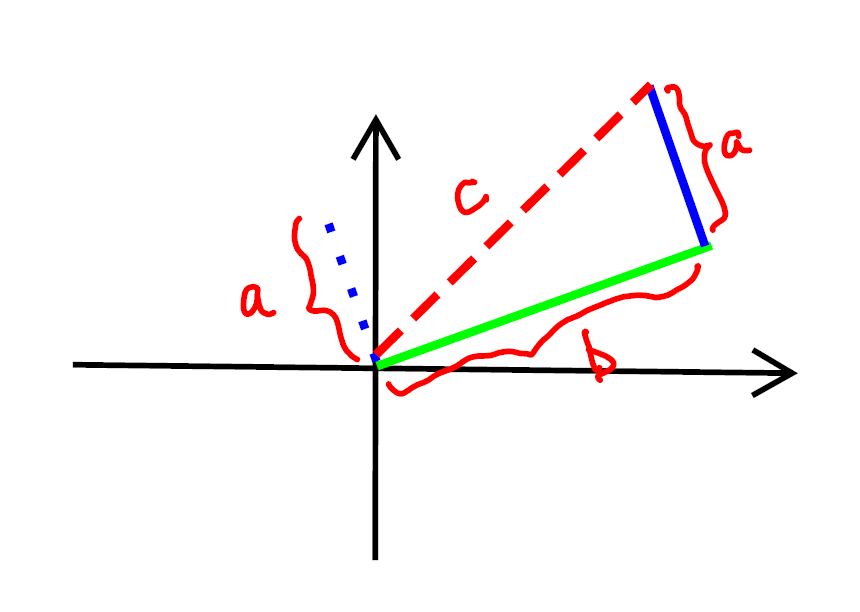
\includegraphics[width=0.35\textwidth]{graphics/Chap09VectorSpaceRnPart2/RightTriangle.png}
}
\hspace{5pt}%
\subfloat[]{%
    \label{fig:RightTriangle02}%
	\centering
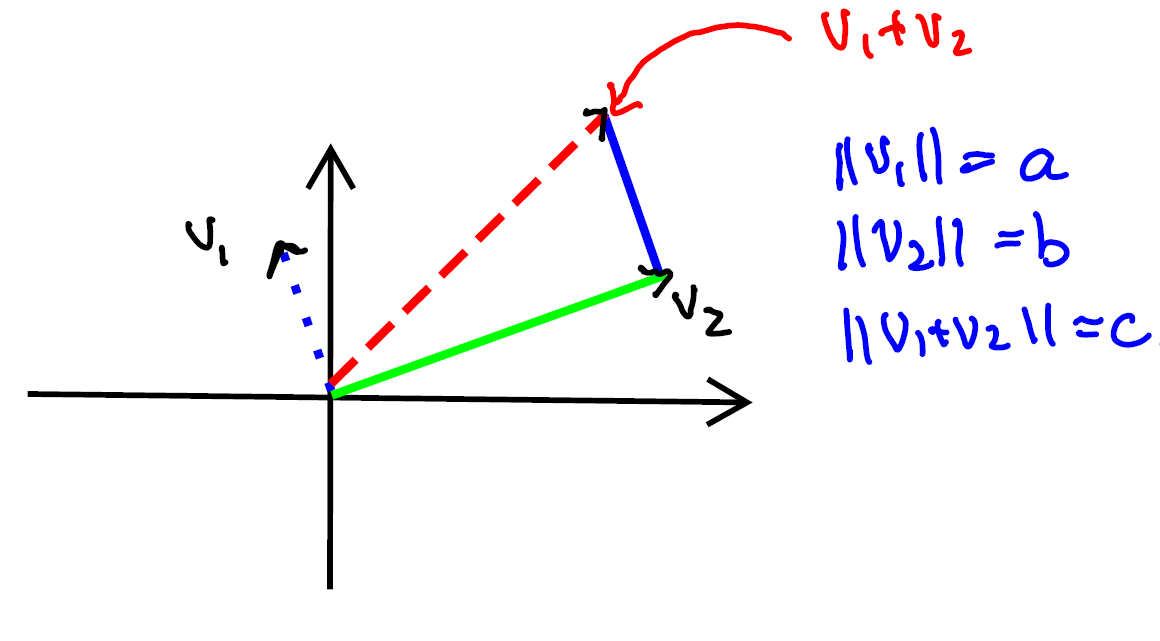
\includegraphics[width=0.45\textwidth]{graphics/Chap09VectorSpaceRnPart2/RightTriangle02.png}}%
\caption[]{How do we go from right triangles to orthogonal vectors satisfying $v_1 \bullet v_2 = 0$?}
    \label{fig:RightTriangle}
\end{figure}

Earlier in the Chapter, we defined two vectors to be orthogonal if their dot product was zero. That's fine, we can make any definition we want, but does this really correspond to our notion of perpendicular vectors? It does, and we can prove that here if you accept that the triangle in Fig.~\ref{fig:RightTriangle}-(a) is a right triangle if, and only if, the Pythagorean Theorem holds, that is, $a^2 + b^2 = c^2 \iff$ the triple $(a,b,c)$ forms a right triangle. In the following we take this as a given. You may need to go back to a High School Geometry book to find this fact.\\


Fig.~\ref{fig:RightTriangle}-(b) interprets the three sides of the triangle in terms of vectors $v_1$, $v_2$, $v_3$ and their norms. We seek to understand the relation that must hold between these vectors for the Pythagorean Theorem to hold. We note that
\begin{equation}
    \begin{aligned}
    ||v_1 + v_2||^2 & := (v_1 + v_2)^\top (v_1 + v_2) \\
    & = v_1^ \top v_1 + v_1^\top v_2 + v_2^\top v_1 + v_2^\top v_2\\
    & ~~~~~~ v_1^\top v_1 +  v_2^\top v_2 + 2 v_1^\top v_2 \\
    & =: ||v_1||^2 + ||v_2||^2 + 2 v_1 \bullet v_2.
    \end{aligned}
\end{equation}
Hence, 
$$\text{Pythagorean Theorem holds } \iff \left(||v_1 + v_2||^2 = ||v_1||^2 + ||v_2||^2 \right) \iff  v_1 \bullet v_2 =0 \iff v_1 \perp v_2,$$
which is what we wanted to show!\\

\begin{tcolorbox}[title={\bf How general do you want to go?}]
      The notions of inner products and orthogonality can be greatly extended. We have merely scratched the surface here. ROB 501 explores these topics in great detail. You may also enjoy this YouTube video by Michael Penn: \url{https://youtu.be/Dz_tsaocWek}. He has a massive channel full of Math videos: \url{https://www.youtube.com/@MichaelPennMath}.  
\end{tcolorbox}


\section{Looking Ahead}

We will complete our introduction to Linear Algebra by introducing you to eigenvalues and eigenvectors. We'll also apply to matrices the concepts of subspace and dimension. This will give us a more complete understanding of solutions to systems of linear equations.